% To compile, make sure to have the following packages installed:
% texlive, texlive-latex-extra, texlive-science, 
% texlive-fonts-recommended, texlive-fonts-extras

\documentclass[journal]{IEEEtran}
%\documentclass{article}
\usepackage{footnote}
\usepackage{multirow}
%\usepackage[font={small}]{caption}
%\usepackage{sidecap}
\usepackage{graphicx}
\usepackage{cite}
\usepackage[draft]{hyperref}
%\usepackage[options]{nohyperref}
%\usepackage{url}
%\usepackage[stable]{footmisc}
%\usepackage{caption}
%\usepackage{adjustbox}
\usepackage{subcaption}
\usepackage{algpseudocode}
\usepackage{algorithm}
\usepackage{amsmath}
\usepackage{amssymb}
\usepackage{bbm}
\usepackage[T1]{fontenc}
\usepackage[utf8]{inputenc}
%\usepackage{authblk}
\pdfminorversion=4
\DeclareMathOperator*{\argmax}{arg\,max}
\DeclareMathOperator*{\argmin}{arg\,min}

\newcommand{\twopartdef}[4]
{
	\left\{
		\begin{array}{ll}
			#1 & \mbox{if } #2 \\
			#3 & \mbox{if } #4
		\end{array}
	\right.
}

\title{A decade of lost precision: Introducing a general framework for 
image feature matching without geometric constraints}

\author{%
\IEEEauthorblockN{%
Jonas Toft Arnfred,\IEEEauthorrefmark{1} Stefan 
Winkler,\IEEEauthorrefmark{1} Sabine S\"usstrunk\IEEEauthorrefmark{2}}\\
\vspace{1mm}
\IEEEauthorblockA{%
\IEEEauthorrefmark{1}~Advanced Digital Sciences Center (ADSC), University of Illinois at Urbana-Champaign (UIUC), Singapore\\
\IEEEauthorrefmark{2}~\'Ecole Polytechnique F\'ed\'erale de Lausanne (EPFL), Switzerland}
}

\begin{document}
\maketitle
%
\begin{abstract}
Solutions in computer vision involving the matching of local image 
features frequently use \emph{Ratio-Match} as introduced by Lowe and 
others, but is this really the best approach? We formalize the 
theoretical foundation of \emph{Ratio-Match} and propose a general 
framework encompassing \emph{Ratio-Match} and three other matching 
methods. Using the framework we establish a theoretical order of 
performance in terms of precision and recall between the methods and 
prove that \emph{Ratio-Match} is consistently equalled or outperformed 
by all other methods of the framework.

We confirm the theoretical results experimentally on over 3000 image 
pairs and show that we can easily increase matching precision
without further assumptions about the images we are using. These gains 
comes without increased computation time by changing only a few key 
components of the \emph{Ratio-Match} algorithm.

\end{abstract}
%
\section{Introduction}
%
Matching image points is a crucial ingredient in almost all computer 
vision algorithms that deal with sparse local image features. This 
includes image categorisation \cite{bosch2008scene}, image stitching 
\cite{brown2007automatic}, object detection \cite{zhang2007local} and 
near duplicate detection \cite{zhao2009scale} to mention a few examples.  
These problems all rely on being able to accurately find the 
correspondence(s) of a point on an object in a \emph{query image} given 
one or more \emph{target images} that might contain the same object.  In 
many applications the target images have undergone transformations with 
respect to the query image; in stereo vision, the camera angle is 
different, while in object recognition and near duplicate detection both 
the lighting and even the object itself can also be transformed.

In the literature two approaches to feature point matching have been 
pursued and later merged. The geometric approach tries to find unique 
keypoints in an image pair and match them based on their location.  The 
descriptor centric approach on the other hand uses the local image 
information around the keypoint to create a descriptor and match 
descriptors based on their similarity.

In the purely geometric approach we try to consistently match feature 
points based on their position in the images. Scott and Longuet-Higgins 
\cite{scott1991algorithm} and Shapiro and Brady 
\cite{shapiro1992feature} introduced the use of spectral methods by 
deriving a coherent set of matches from the eigenvalues of the 
correspondence matrix. Other examples of this approach include Sclaroff 
and Pentland \cite{sclaroff1995modal} as well as Carcassoni and Hancock 
\cite{carcassoni2003spectral}.

The descriptor centric approach on the other hand finds matches by 
pairing keypoints from locations where the images are similar. The first 
examples of this approach used the correlation of the raw image data 
immidiately surrounding the feature point \cite{deriche1994robust}, 
\cite{baumberg2000reliable} to calculate this similarity. Later 
algorithms were enhanced by creating invariant feature descriptors first 
introduced in \cite{schmid1997local} and later popularized by the work 
of Lowe introducing SIFT \cite{lowe2004sift} and Bay introducing SURF 
\cite{bay2006surf}.

Many descriptor variations have since been proposed and a few surveys 
have emerged comparing them. Mikolajczyk and Schmid evaluates 11 such 
feature descriptors in a paper where they also introduce the graffiti 
image set which has later become a common benchmark for image matching 
algorithms \cite{mikolajczyk2005performance}.  Later Moreels and Perona 
evaluated 5 descriptors with different keypoint detectors using a large 
image set consisting of 3D models \cite{moreels2007evaluation}. Finally 
Heinly et al.\ take a closer look at binary features such as BRIEF 
\cite{calonder2010brief}, BRISK \cite{leutenegger2011brisk} and ORB 
\cite{rublee2011orb} comparing them to SIFT and SURF 
\cite{heinly2012comparative}. 

A straightforward way to find a set of correspondences using only 
feature points is to threshold the similarity measure of the feature 
vectors, accepting only correspondences that score above a certain 
threshold \cite{szeliski2010}. When we match images with the assumption 
that the correspondence between two feature points will be unique we can 
further increase precision by only matching a feature point to its 
nearest neighbor in terms of descriptor similarity. Instead of 
thresholding based on similarity, Deriche et 
al.~\cite{deriche1994robust} and Baumberg~\cite{baumberg2000reliable} 
propose using the ratio of the similarity of the best to second best 
correspondence of a given point to evaluate how unique it is. Their 
finding has later been tested by several independent teams, all 
concluding that thresholding based on the ratio is generally superior to 
thresholding on similarity \cite{lowe2004sift}, 
\cite{mikolajczyk2005performance}, \cite{moreels2007evaluation}, 
\cite{rabin2009statistical}. Brown and Lowe extends ratio match to deal 
with a set of images by using not the ratio of the best and second best 
correspondence, but the average ratio of the best and the average of 
second best correspondences across a set of images 
\cite{brown2005multi}.  Rabin et al.\ tries to enhance descriptor 
matching by looking at the statistical distribution of local features in 
the matched images, and only return a correspondence when such a 
correspondence would not occur by mere chance 
\cite{rabin2009statistical}. Finally, a precursor of the algorithms 
discussed in this paper were introduced by the authors as 
\emph{Mirror-Match} \cite{arnfred2013mirror} which makes use of the 
feature points in both images to decide if a match is valid.

A plethora of solutions have combined ratio match with various geometric 
constraints to improve matching. These constraints are based on 
assumptions regarding the transformation between the query and target 
images. At the stricter end we have epipolar constraints assuming
that the images can be tied by a homography \cite{torr2000mlesac}, 
\cite{chum2005matching} and angular constraints assuming the 
correspondences are angled similarly \cite{kim2008efficient}, 
\cite{schmid1997local}. Often these approaches are made computationally 
feasible by modelling the case of feature correspondences as an instance 
of graph matching where each feature is a vertex and edge values 
correspond to a geometric relation between two features. In this case 
approximate graph matching algorithms can be used to efficiently 
establish an isomorphism between the graph of features in two images 
\cite{leordeanu2005spectral}, \cite{torresani2008feature}, 
\cite{yarkony2010covering}. Finally others define image regions and 
reject or accept correspondences based on the regions they connect 
\cite{cho2009feature}, \cite{wu2011robust}.

Any matching method relying on geometric constraints is restrained by an
inherent assumptions about the geometric relationship between the two 
images. Broad assumptions such as angular constraints often used in 
graph matching only apply to simple image transformations. For more 
complex transformations we need models suitable for each particular case 
and hence limit the algorithm to the subset of images that fit the 
model. In the case of object recognition for example, the 
transformations from one scene to another often feature a change in 
perspective, background and sometimes variations within the object 
itself. In most circumstances this makes these methods unsuited for 
epipolar or angular constraints.

If we intent to match these instances using geometric features we are 
forced to used a sophisticated model that reflects the variations in 
which we find these objects, an in the process lose generality. For this 
reason general descriptor based algorithms are crucial for 
correspondence applications calling for generality. In addition the 
advantage of purely descriptor based methods is motivated by the fact 
that any geometric method acts as a filter on a given set of 
correspondences.  If this set contains less incorrect correspondences, 
the final set can be calculated faster and more accurately.

The methods we propose in this paper are designed to be free of 
assumptions about image geometry. They extend and improve on Lowe's 
\emph{Ratio-Match} \cite{lowe2004sift} and the author's \emph{Mirror 
Match} \cite{arnfred2013mirror} by generalizing both algorithms to a 
framework of matching methods. We go on to formally establish an order 
comparing how well different methods within the framework compares in 
terms of precision and recall. Our experimental evaluations confirm the 
theoretical results and show that \emph{Ratio-Match} on all counts is a 
unoptimal choice as a matching algorithm independent of application. 

In the author's last paper we introduced \emph{Mirror-Match} and 
\emph{Mirror-Match with Clustering}, two algorithms that we showed to 
perform better than the state of the art. The novel contributions of 
this paper consists of two new algorithms completing a framework of four 
related matching algorithms as well as the theoretical foundation which 
enables us to understand why \emph{Mirror-Match} performs better than 
\emph{Ratio Match} in the first place.

The paper is organized as follows. I section~\ref{S:MatchingMethods} we 
introduce the original \emph{Ratio-Match}, extend on this method to 
introduce the proposed framework and go on to compare the members of the 
framework theoretically.  In section~\ref{S:Experiments} we present 
evaluations and discuss the results obtained.  Section~\ref{S:Summary} 
concludes the paper.

\section{Matching Methods}
\label{S:MatchingMethods}
%
\subsection{Ratio-Match}
%
\emph{Ratio-Match} as introduced by Deriche et al.
\cite{deriche1994robust} and later used by 
Baumberg~\cite{baumberg2000reliable} and Lowe~\cite{lowe2004sift} makes 
use of a \emph{uniqueness ratio}. For each feature in the \emph{query 
image} we find a possible match by identifying the nearest neighbor and 
returning this match only if the \emph{uniqueness ratio} is above a 
given threshold, $\tau$. Given $f_q$, a feature from the \emph{query 
image} and $F_{target}$, a set of features from the \emph{target image}, 
the nearest neighbor of $f_q$ in $F_{target}$ is:
\begin{equation*}
    \argmin_{f_t \in F_{target}} d(f_q, f_t)
\end{equation*}
Here, $d(f_i, f_j)$ is the distance between the feature descriptors.  
With SIFT and SURF this is the euclidian distance of the feature vectors
\cite{lowe2004sift} \cite{bay2006surf} where as BRIEF, BRISK and FREAK 
measure the distance as the hamming distance \cite{leutenegger2011brisk} 
\cite{calonder2010brief} \cite{alahi2012freak}.  If we let $f_p$ and 
$f_b$ be the nearest and second nearest neighbor of a feature, $f_q$, 
the \emph{uniqueness ratio} is defined as follows:
\begin{equation*}
    r = d(f_q, f_p) / d(f_q, f_b)
\end{equation*}
Because $f_p$ is the nearest neighbor and $f_b$ the second nearest 
neighbor we know that $d(f_q, f_p) \leq d(f_q, f_b)$ and since $d(f_i, 
f_j) \geq 0, \forall f_i,f_j$, the uniqueness ratio is bounded by $0$ 
and $1$, both inclusive. For the degenerate case where $d(f_q, f_b) = 0$
we let the \emph{uniqueness ratio} be $0$.

The underlying assumption in ratio match is that the point we seek to 
match in the \emph{query image} has only one match in a given 
\emph{target image} or no matches at all. In both cases should expect 
that the \emph{second} nearest neighbor in the target image to be an 
untrue correspondence.  This means we can use the distance between the 
feature point and the second closest descriptor as a \emph{baseline} for 
false correspondences. By dividing the distance to the nearest neighbor 
with this baseline we get an estimated measure for how distinct the 
correspondence is from a false match.  

To make further discussion easier we introduce the following 
nomenclature:

\begin{itemize}
\item{Let $f_q$ be any feature point in the \emph{query image} that we 
    are currently trying to match}
\item{Let $F$ be a set of features. $F_{target}$ for example is the set 
    of features from the \emph{target image}}
\item{Let $\tau \in [0 \ldots 1]$ be a threshold used to decide whether 
    to keep a match or discard it. We keep a match only if is has a 
\emph{uniqueness ratio} lower than $\tau$}
\item{Let the \emph{proposed match} be the nearest neighbor of the query 
    feature $f_q$ picked from a set of feature points that we will call 
the \emph{proposal set} which does not contain the query feature itself}
\item{Let the \emph{baseline match} be the nearest neighbor of the query 
    feature $f_q$ picked from a set of feature points that we will call 
the \emph{baseline set} which neither contains the \emph{proposed match} 
nor the query feature}
\end{itemize}

%
\subsection{A framework of matching methods}
%

\begin{figure}[t]
\centering
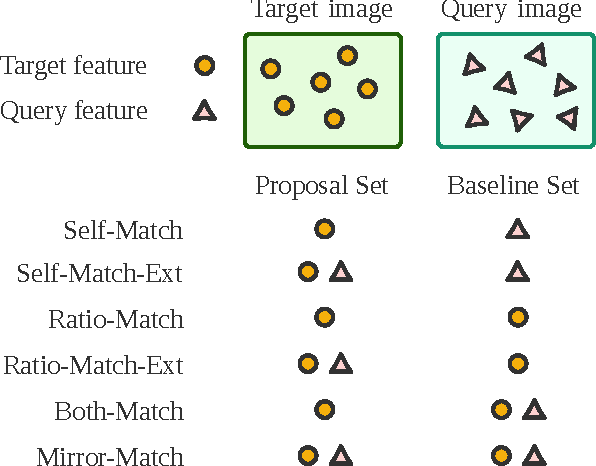
\includegraphics[width=0.85\columnwidth]{images/overview}
\caption{Graphical representation of the \emph{Baseline} and 
\emph{Proposal Set} for different methods in the proposed framework}
\label{fig:overview}
\end{figure}

Given two images we can construct the proposal and baseline sets in six 
different ways as illustrated in Figure~\ref{fig:overview}. In the case 
of \emph{Ratio-Match} \cite{lowe2004sift} the \emph{proposal set} 
consists of all the feature points in the target image.  Similarly the 
\emph{baseline set} consists of all the feature points in the target 
image except the \emph{proposed} match. For \emph{Ratio-Match} this 
practically means that given a query feature, $f_q$, the \emph{proposed 
match} and the \emph{baseline match} are the two nearest neighbors in 
the set of feature points in the \emph{target image} and the ratio is 
decided uniquely based on the \emph{target image}. In turn 
\emph{Mirror-Match} as introduced by the authors in 
\cite{arnfred2013mirror}, works by constructing the \emph{proposal set} 
and \emph{baseline set} by combining features from both the \emph{query} 
and \emph{target image}. By similar variations of the \emph{proposal} 
and \emph{baseline set} we derive four more algorithms as illustrated in 
Figure~\ref{fig:overview}, however we will not discuss 
\emph{Self-Match-Ext} and \emph{Both-Match} further in this paper since 
we show them to be equivalent with \emph{Self-Match} and 
\emph{Mirror-Match} respectively in Appendix~\ref{A:self} and 
\ref{A:mirror}.

\begin{algorithm}[htb]
\caption{Generalized matching algorithm for two images}
\label{alg-gen}
\begin{algorithmic}
    \Require $I_{query}, I_{target}$ : images, $\tau \in [0,1]$
    \State $F_{query} = get\_features(I_{query})$
    \State $F_{target} = get\_features(I_{target})$
\State $F_{proposal-all} = get\_proposal\_features(F_{query}, 
F_{target})$
\State $F_{baseline-all} = get\_baseline\_features(F_{query}, 
F_{target})$
\State $M = \varnothing$
\ForAll{$f_q \in F_{query}$}
    \State $F_{proposal} = F_{proposal-all} \setminus 
    \left\{f_q\right\}$
    \State $F_{baseline} = F_{baseline-all} \setminus \left\{f_q, 
    f_p\right\}$
    \State $f_p \gets getNearestNeighbo\text{r}(f_q, F_{proposal})$
    \State $f_b \gets getNearestNeighbo\text{r}(f_q, F_{baseline})$
    \State $ratio \gets distance(f_q, f_p) / distance(f_q, f_b)$
    \If{$(ratio < \tau) \wedge (f_p \in F_{target})$}
        \State $matches \gets matches \cup \left(f_q, f_p\right)$
	\EndIf
\EndFor
\Return $M$
\end{algorithmic}
\end{algorithm}

In algorithm~\ref{alg-gen} we show the generalized matching framework 
where the \emph{proposal set} and \emph{baseline set} are defined 
according to Figure~\ref{fig:overview}.  In practice for i.e.\ 
\emph{Ratio-Match} we can obtain $f_p$ and $f_b$ by finding the 2 
nearest neighbors of $F_{target}$. The other algorithms can be optimized 
similarly. In Figure~\ref{fig:matching} we illustrate the structure of 
this algorithm.

For methods where the \emph{proposal set} includes the \emph{query 
features} it is possible that the \emph{proposal match} is a feature 
from the \emph{query image}, in which case we discard the match as an 
untrue correspondence.  It also happens that we encounter 
correspondences where the uniqueness ratio is more than $1$ in which 
case we set it to $1$ to maintain a bounded \emph{uniqueness ratio}.  
Take for example the case of \emph{Self-Match}. Using this method we 
might find that the nearest neighbor of a feature in the target image is 
further from the query feature than the nearest neighbor in the query 
image. In this case the match is discarded.

%
\subsection{Generalized Uniqueness Ratio}
%

\begin{figure}[t]
\centering
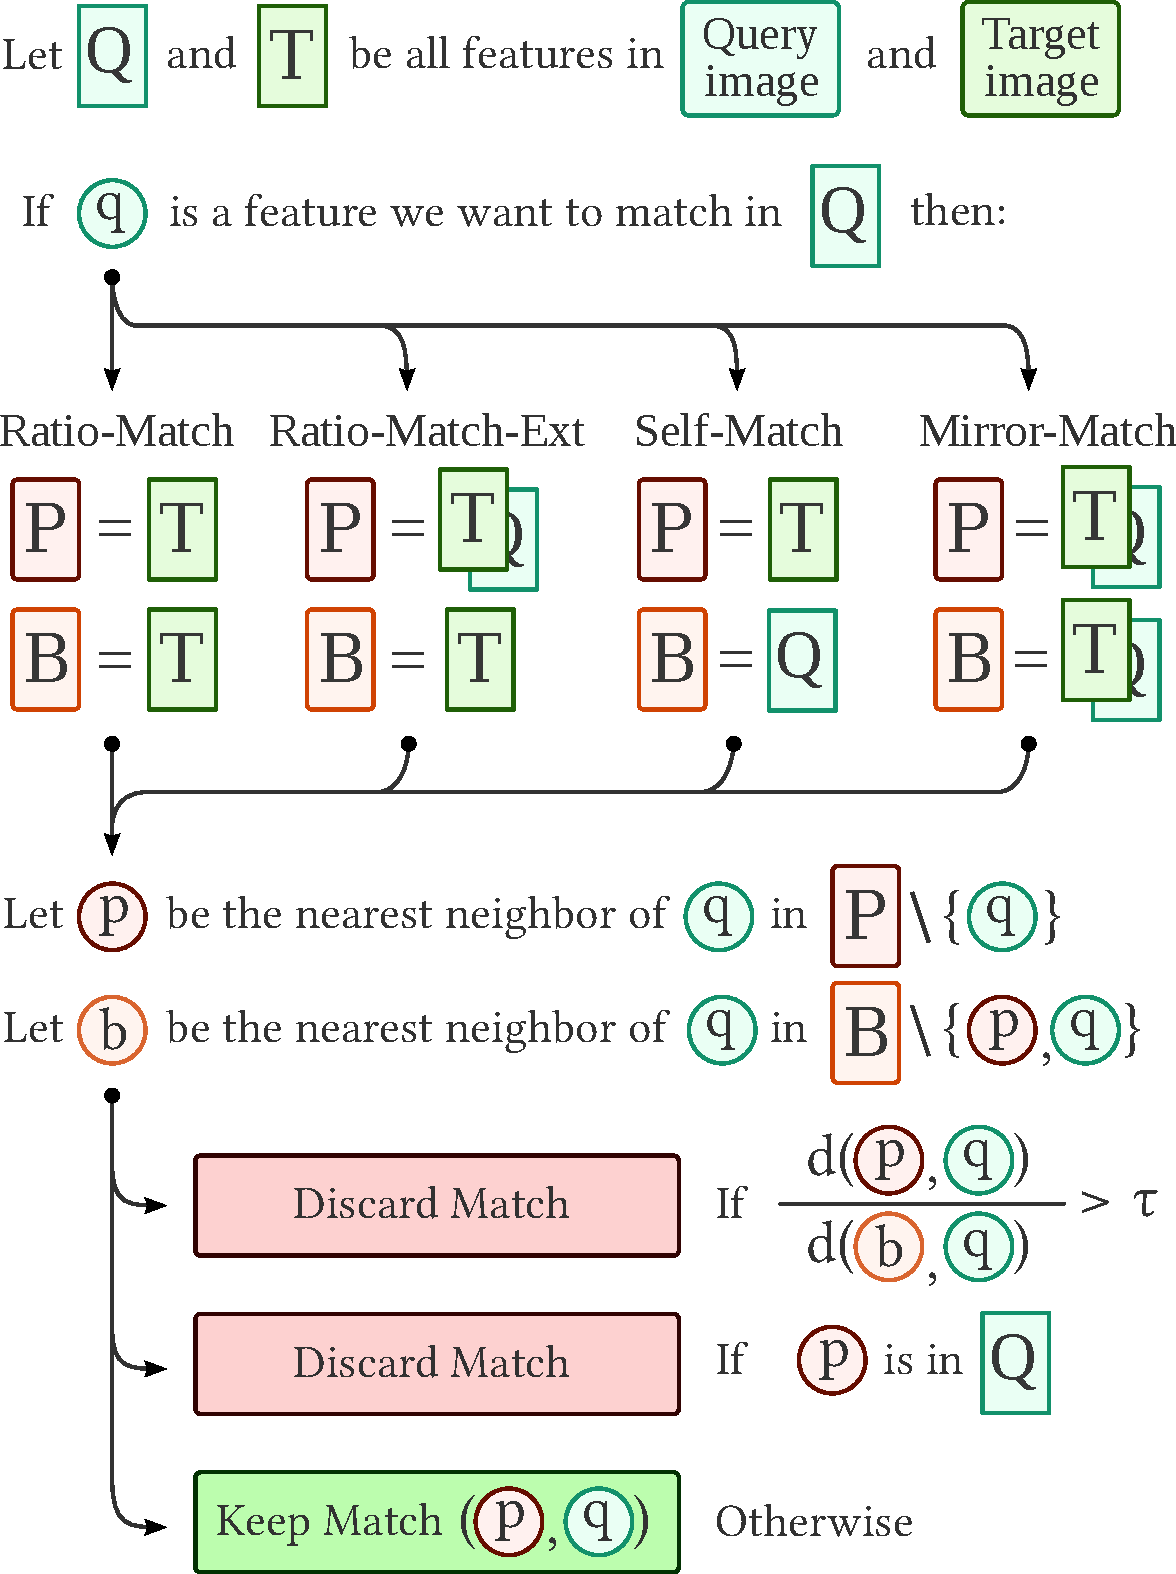
\includegraphics[width=0.9\columnwidth]{images/matching}
\caption{Flow chart showing what happens when we match a feature. $\tau$ 
is the ratio threshold and $d(x,y)$ is the distance between two feature 
descriptors, $x$ and $y$.}
\label{fig:matching}
\end{figure}
%

The main distinguishing factor in between the algorithms in the 
framework is the final ratio between the distance of the two nearest 
neighbors of a query feature which decides if we keep or discard a 
match. We illustrate this process in Figure~\ref{fig:matching}. 

We can define a calculation of this ratio common to all algorithms in 
the framework which allows us to compare the algorithms theoretically. 
The theoretical ratio, $r$ is defined as follows:

If $f_{p}$ is the nearest neighbor of $f_{q}$ in $F_{proposed}$ and 
$f_{b}$ is the nearest neighbor of $f_{q}$ in $F_{baseline} \setminus 
\left\{f_{p}\right\}$ then the generalized \emph{uniqueness} ratio is:
\begin{align*}
    r &= \text{r}(f_{q}, F_{proposed}, F_{baseline}) \\
        &= \frac{d(f_{q}, f_{p})}{d(f_{q}, f_{b})}
\end{align*}
We let $K$ be the number of possible true correspondences \emph{query} 
and \emph{target image}. The \emph{precision} and \emph{recall} are then 
defined as:
\begin{align*}
    \textrm{Recall} &= \frac{\#\textrm{Correct Matches}}{K} \\
    \textrm{Precision} &= \frac{\#\textrm{Correct 
    Matches}}{\#\textrm{Correct Matches} + \#\textrm{Incorrect Matches}}
\end{align*}
Given $f_{nn} \in F_{target}$ defined as the nearest neighbor of any 
$f_q \in F_{query}$ then we define the set of features $F_{true}$ as 
$\left\{ f_{q} \in F_{query} \mid f_{nn} \text{ is a true correspondence 
of } f_{q} \right\}$ and $F_{false}$ as $F_{query} \setminus F_{true}$.  
We can the define the number of correct and incorrect matches as 
follows:
\begin{align*}
    \textrm{keep\_match}(f_{q}) &= \twopartdef{ 1 }{\text{r}(f_{q}, 
    F_{proposed}, F_{baseline}) <
    \tau}{0}{\textrm{otherwise}} \\
    \#\textrm{Correct Matches} &= \sum_{f_{q} \in F_{true}} 
    \textrm{keep\_match}(f_{q})\\
    %\mathbbm{1}_{\left\{ \right\}} \\
    \#\textrm{Incorrect Matches} &= \sum_{f_{q} \in F_{false}}
    \textrm{keep\_match}(f_{q})
    %\mathbbm{1}_{\left\{ r < \tau\right\}}
\end{align*}

From the above we can conclude that the performance in terms of 
precision and recall of any method from the proposed framework is 
uniquely identified by the uniqueness ratio $r$.  If for every query 
feature $f_{q}$, $r$ is identical across two matching methods, then they 
return identical results. 

\subsection{Proofs of Ordering}

Under three assumptions that largely reflects the performance of 
matching feature points in practice we can theoretically compare the 
performance of the different algorithms shown in 
Figure~\ref{fig:overview}.

\begin{enumerate}
    \item{For a query and target image we assume that for any point in 
        the query image there is at most one real correspondence in the 
    target image and no real correspondences in the query image itself 
as assumed by \emph{Ratio-Match}}
    \item{We assume that distances of feature descriptors are well 
            behaved.  More precisely, given $f_q$, a feature from the 
            \emph{query image} and $f_{match}$, the real correspondence 
            from the set of features in the \emph{target image} 
            $F_{target}$, we have that $\forall f_i \in F_{proposal}, 
            f_i \neq f_{match}: d(f_q,f_{match}) < d(f_q, f_i)$}
    %\item{We assume that features within one image resemble each other 
            %more than features in different images. That is, given 
            %$f_a,
    %        f_i \in F_1$ and $f_b, f_j \in F_2$ where $(f_i, f_j)$ and 
    %    $(f_a, f_b)$ are true correspondences, and $F_1$ and $F_2$ are 
    %features collected from different images then we expect that 
            %$d(f_a, f_i)% < d(f_a, f_j)$ and $d(f_b, f_j) < d(f_b, 
            %f_i)$}
     \item{For a set of query features $F_{query}$ with a true 
             correspondence in the \emph{target image}, we assume that 
             the distribution of uniqueness ratios using $F_{target}$ as 
             the baseline set is similar to using $F_{query}$, since the 
         two images in the case of true correspondences are guaranteed 
     to share part of the same scene.}
    \end{enumerate}

Based on these assumptions we prove that \emph{Ratio-Match-Ext} is equal 
or better than \emph{Ratio-Match} in terms both precision and recall.  
Consider the nearest neighbor $f_{nn}$ of a query feature $f_{q}$ and 
the two cases where we either have the $f_{nn} \in F_{query}$ or $f_{nn} 
\in F_{target}$. For $f_{nn} \in F_{target}$ the uniqueness ratio of 
\emph{Ratio-Match-Ext} is:
\begin{align*}
    r &= \text{r}(f_{q}, F_{proposed}, F_{baseline}) \\
        &= \text{r}(f_{q}, F_{query} \cup F_{target}, F_{baseline})\\
        &= \text{r}(f_{q}, F_{target}, F_{baseline})
\end{align*}

Since $F_{proposed} = F_{target}$ for \emph{Ratio-Match} this shows that
when the nearest neighbor is found in the target image, the two 
algorithms behave identically. For $f_{nn} \in F_{query}$ 
\emph{Ratio-Match} gives us the following ratio:
\begin{align*}
    r &= \text{r}(f_{q}, F_{proposed}, F_{baseline}) \\
        &= \text{r}(f_{q}, F_{target}, F_{target})
\end{align*}


That is, \emph{Ratio-Match} calculates the ratio based on the two 
nearest correspondences in the \emph{Target Image}. 
\emph{Ratio-Match-Ext} on the other hand does not return any 
correspondence because the nearest neighbor is in the \emph{Query 
Image}. Since query features with a nearest neighbor in the \emph{query 
image} are false correspondences per assumption \#1 and \#2, this proves 
that \emph{Ratio-Match-Ext} has superior \emph{Precision} to 
\emph{Ratio-Match} while maintaining equal \emph{Recall}.

Next we show that \emph{Mirror-Match} is equal or better than 
\emph{Ratio-Match-Ext} in terms of precision and recall. Consider as 
before the nearest neighbor $f_{nn}$ of a query feature $f_{q}$. When 
$f_{nn}$ resides in the \emph{query image} both algorithms behave alike 
and discard the match.  However, consider the uniqueness ratio of 
\emph{Mirror-Match} for the case where $f_{nn}$ resides in the 
\emph{target image}:
\begin{align*}
    r &= \text{r}(f_{q}, F_{proposed}, F_{baseline}) \\
        &= \text{r}(f_{q}, F_{proposed}, F_{query} \cup F_{target})\\
        &= max( \text{r}(f_{q}, F_{proposed}, F_{target}), 
    \text{r}(f_{q}, F_{proposed}, F_{query}) )
\end{align*}

For a true correspondence we have that the uniqueness ratio using 
$F_{query}$ as baseline is distributed similarly to the ratio when using 
$F_{target}$ by assumption \#3. In this case the algorithm performs like 
\emph{Ratio-Match-Ext}.  However for an untrue correspondence with a 
baseline match in the query image which is closer than the
baseline match in the target image, \emph{Mirror-Match} will return a 
worse uniqueness ratio. This in turns means that \emph{Mirror-Match} is 
equal or better than \emph{Ratio-Match-Ext} in terms of  
\emph{Precision} while maintaining equal \emph{Recall}.

Using a similar procedure we prove that \emph{Self-Match} is equal to
\emph{Self-Match-Ext} and \emph{Both-Match} is equal to \emph{Mirror
Match} in Appendix~\ref{A:self} and \ref{A:mirror} respectively.

For any given recall we have proven based on assumption \#1-3 that the 
precision of the algorithms in the framework compares as follows:
\begin{align*}
    \textit{Ratio-Match} &\leq \textit{Ratio-Match-Ext} \leq 
    \textit{Mirror-Match}
\end{align*}

The difference between \emph{Self-Match} and \emph{Ratio-Match} is
the source of the \emph{baseline set}. For true correspondences we 
assume that they should perform similarly but as for the rest the 
performance of the two depends entirely on the images we are matching. 
When we match images where the target image might not overlap at all 
with the query image, using the query image and not the target image as 
a \emph{baseline set} seems like a reasonable choice given that the 
baseline set in this case would be closer to the feature matched and 
more strictly rule out untrue correspondences.


\subsection{Discussion of assumptions}
\label{ref:disc_assumptions}

% Assumption 1
%For a query and target image we assume that for any point in the query 
%image there is at most one real correspondence in the target image and 
%no real correspondences in the query image itself as assumed by 
%\emph{Ratio-Match}

% Assumption 2
%We assume the distances of feature descriptors behave in a \emph{nice} 
%manner. That is, given $f_q$, a feature from the \emph{query image} and 
%$f_{match}$, the real correspondence from the set of features in the 
%\emph{target image} $F_{target}$, we have that $\forall f_i \in 
%F_{proposal}, f_i \neq f_{match}: d(f_q,f_{match}) < d(f_q, f_i)$

% Assumption 3
%For a query feature, $f_q$ with a true correspondence in the 
%\emph{target image}, we assume that the uniqueness ratio using 
%$F_{target}$ is similar to the uniqueness ratio using $F_{query}$, 
%since the two images in this case are guaranteed to share part of the 
%same scene

The three assumptions proposed in order to formalize the order of the 
algorithms have been chosen to reflect conditions under which we ideally
would match feature points. However, for each assumption there exists 
corner cases where it is no longer valid. In this section we intent to 
discuss these corner cases in order to give an impression of the 
circumstances under which the absolute or relative performance of the 
algorithms might differ.

The first assumption states that there is at most one unique match to 
every feature point which is often the case when in e.g.\ stereo 
matching with natural images. However for recognition of object classes 
or in generated images with repetitive content this assumption is no 
longer valid and using any assumption of uniqueness will lead to 
incorrect results. However, as long as the query image does not contain 
repetitive objects we can still use \emph{Self-Match} without loss of 
precision even if the target image might not contain a unique match.

According to the second assumption, feature descriptors behave such that
when matched, a true correspondence to a query feature will always be 
the nearest neighbor. For actual feature detectors and descriptors 
Mikolajczyk and Tuytelaars shows that this property depends strongly on 
the differences between query and target image 
\cite{mikolajczyk2005performance} \cite{tuytelaars2008local}. In the 
degenerate case where the closest match is not an actual correspondence, 
it is often the case that other matches are similarly close resulting in 
a uniqueness ratio near 1, effectively filtering out bad 
correspondences.  This means that with a lenient threshold close to 1, 
the guarantees about precision and recall equivalence in between the 
different ratio algorithms might no longer hold due to the lack of 
consistent descriptor behaviour. It is worth pointing out that if this 
assumption holds true, matching using only nearest neighbor is not 
necessarily optimal unless there is a complete scene overlap between
the images matched. For cases where there is little or no overlap, a 
nearest neighbor would indiscriminately return false matches even with 
well behaved feature descriptors.

\begin{figure}[t]
\centering
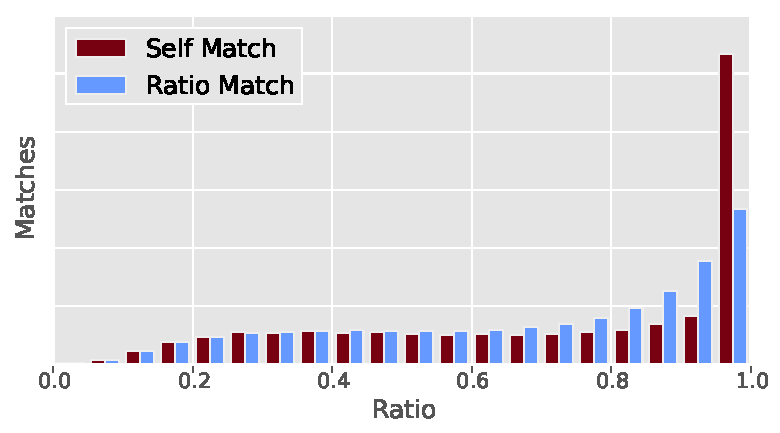
\includegraphics[width=0.99\columnwidth]{images/results_ratio_hist}
\caption{Normalized histogram of the \emph{uniqueness ratios} of true 
correspondences for 84 different 3D objects.}
\label{fig:ratio_hist}
\end{figure}

The last assumption states that the uniqueness ratio using either the 
\emph{query} or target image as the baseline set would be similar
in distribution when we know that the feature point we are matching has 
a true correspondence. For an ideal feature descriptor where any true 
correspondence between two feature points will have a distance of $0$, 
the third assumption is obviously true for any cases where the second 
closest feature point has a true correspondence in the other image. For 
non-ideal feature descriptors where the baseline match has a true 
correspondence in the other image we can verify the assumption by 
looking at the \emph{uniqueness ratio} for a true correspondences when 
it is based on the query image compared to when it is based on the 
target image. To compare we plot the actual \emph{uniqueness ratios} 
measured from $84$ 3D objects in Figure~\ref{fig:ratio_hist}. For ratios 
lower than $0.7$ this is generally the case, but as we approach more 
lenient thresholds the performance of \emph{Mirror-Match} might no 
longer be equal or better than \emph{Ratio-Match-Ext} in terms of 
precision.
% Needs rewording

\section{Experiments and Results}
\label{S:Experiments}
%
\begin{figure}[htb]
    \begin{subfigure}[t]{0.48\columnwidth}
        \centering
        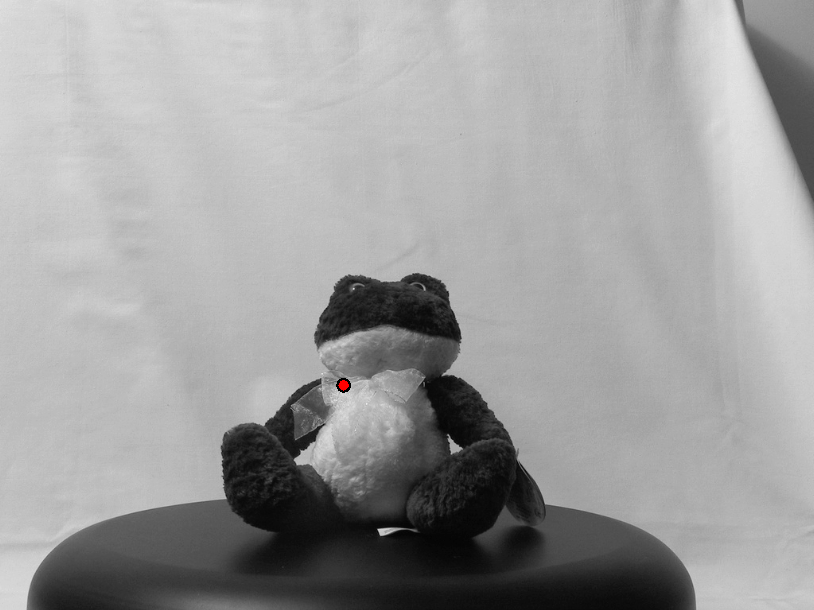
\includegraphics[width=\columnwidth]{images/Frog_A}
        \caption{Query Image}
        \label{fig:frog_a}
    \end{subfigure}%
    \quad %add desired spacing between images, e. g. ~, \quad, \qquad a 
    %blank line to force the subfigure onto a new line)
    \begin{subfigure}[t]{0.48\columnwidth}
        \centering
        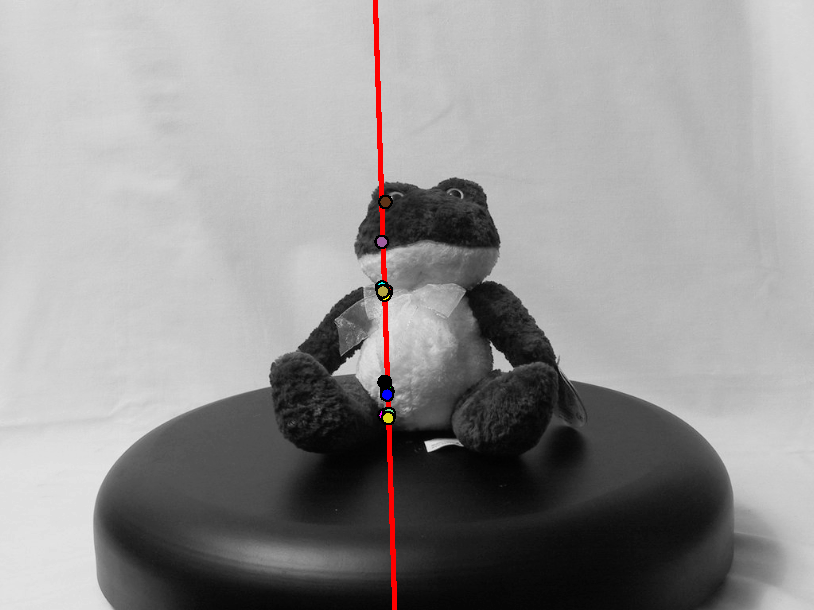
\includegraphics[width=\columnwidth]{images/Frog_B}
        \caption{Auxiliary Image}
        \label{fig:frog_b}
    \end{subfigure}%
    \\ %add desired spacing between images, e. g. ~, \quad, \qquad 
    %a blank line to force the subfigure onto a new line)
    \begin{subfigure}[t]{0.48\columnwidth}
        \centering
        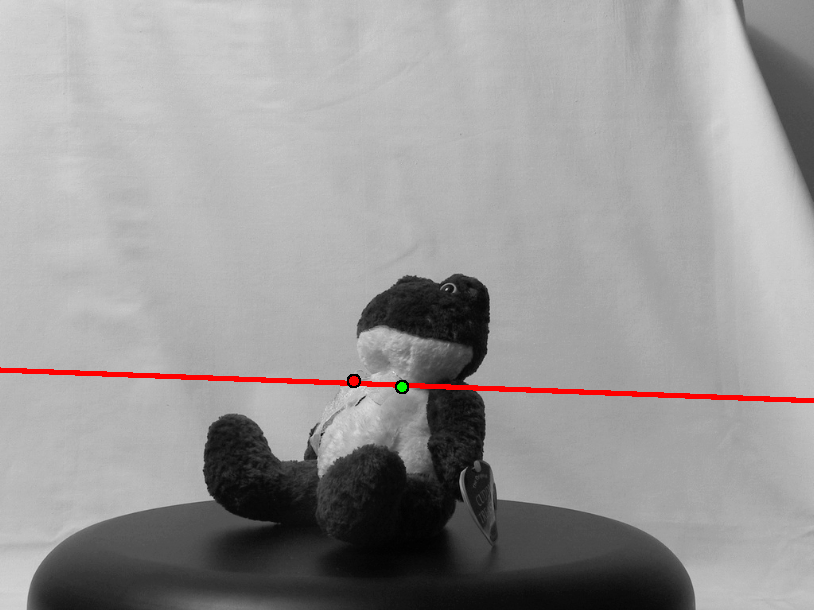
\includegraphics[width=\columnwidth]{images/Frog_C}
        \caption{Target Image}
        \label{fig:frog_c}
    \end{subfigure}%
    \quad %add desired spacing between images, e. g. ~, \quad, \qquad 
    %blank line to force the subfigure onto a new line)
    \begin{subfigure}[t]{0.48\columnwidth}
        \centering
        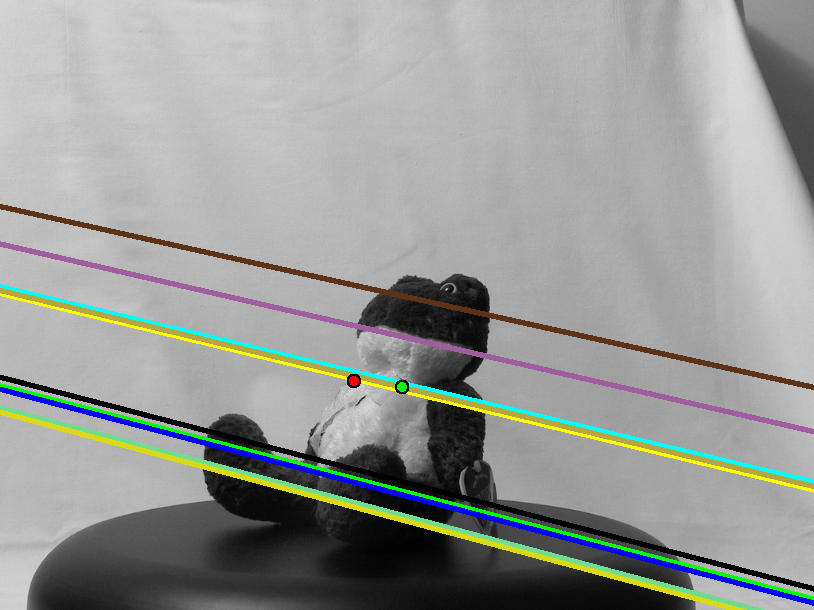
\includegraphics[width=\columnwidth]{images/Frog_C_lines}
        \caption{Target Image with epipolar constraints}
        \label{fig:frog_c_lines}
    \end{subfigure}%
    \caption{Creating epipolar constraints based on three source images.  
        In a) the \emph{query image} has been marked with the position 
        of the feature we are attempting to match. In b) the 
        \emph{auxiliary image} is shown. This image is taken with the 
        same rotation as the \emph{query image} but from a higher 
        viewpoint. The line going through the image is the epipolar line 
        of the feature point in the \emph{query image}.  The markers 
        indicate all feature points in the image found near the epipolar 
        line.  In c) we show the \emph{target image} which in this case 
        is rotated 45 degrees from the \emph{query image}.  The line 
        overlaid on the image represents the epipolar line corresponding 
        to the feature point shown in the \emph{query image}.  The 
        markers indicate all feature points in the image found near the 
    epipolar line. In d) we show the \emph{target image} again, this 
    time overlaid with the epipolar lines corresponding to all the 
    features shown in the \emph{auxiliary image}. A true correspondence 
    should be found within a small distance of one of the intersections 
    of the line in c) and the lines in d). In this particular case both 
    feature points shown in c) and d) could possible be a correct 
    correspondence.
}%
    \label{fig:frog}%
\end{figure}%
In this section we will go over the experimental results comparing 
\emph{Self-Match}, \emph{Ratio-Match}, \emph{Ratio-Match-Ext} and 
\emph{Mirror-Match}. We use two different image databases to compile 
results over different variations.  To measure results on realistic and 
variate non-planar images we test the algorithm on the 3D Objects 
database released by Moreels and Pietro \cite{moreels2007evaluation} in 
Section~\ref{S:3dobjects}. The database contains a set of 86 3D objects 
photographed from all sides at 5 degree intervals from two different 
viewpoints and under three different lighting conditions.

In the experiments we use the \emph{SIFT} descriptor and keypoint 
detector with default parameters as implemented in the OpenCV library 
v.\ 2.4.6.  To test how the framework performs across descriptors we 
evaluate SURF \cite{bay2006surf}, BRISK \cite{leutenegger2011brisk}, 
BRIEF \cite{calonder2010brief} and FREAK \cite{alahi2012freak} in 
Section~\ref{label:desc}. Across all experiments images larger than 
1024x768 have been resized to fit within those dimensions using 
Imagemagick with default parameters and only the luminance channel has 
been used in the feature detection and description stage.

\subsection{Experiments on 3D objects}
\label{S:3dobjects}

\begin{figure}[t]
    \begin{subfigure}[t]{0.19\columnwidth}
        \centering
        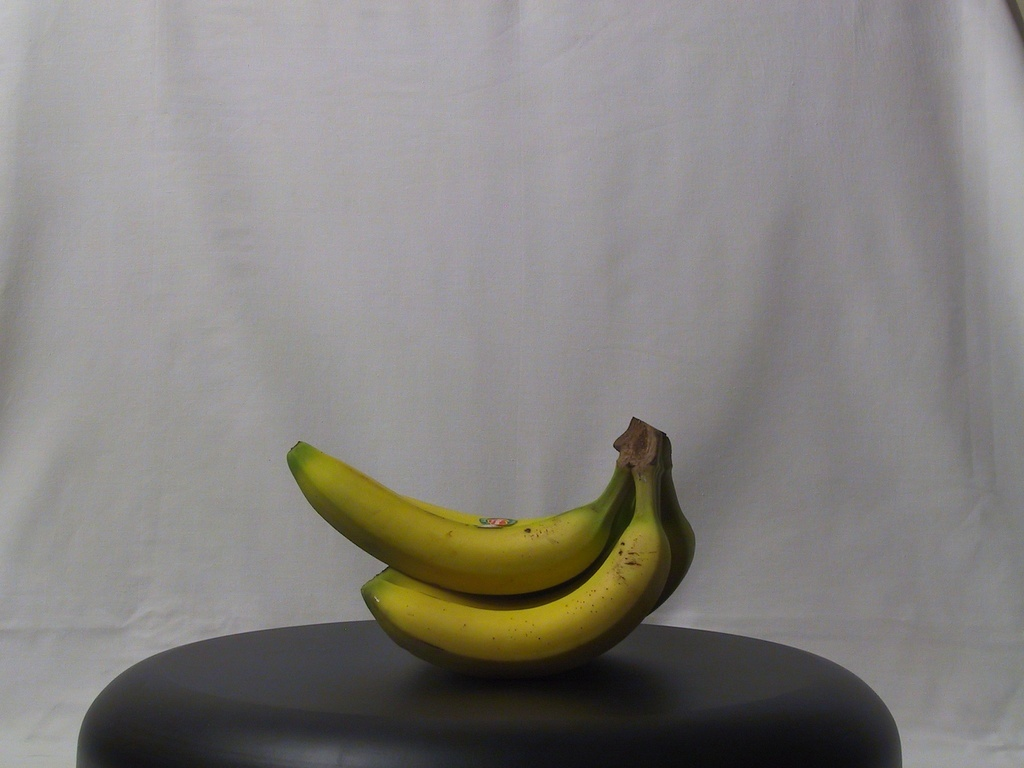
\includegraphics[width=1\columnwidth]{images/3d/1}
    \end{subfigure}%
    ~ %
    \begin{subfigure}[t]{0.19\columnwidth}
        \centering
        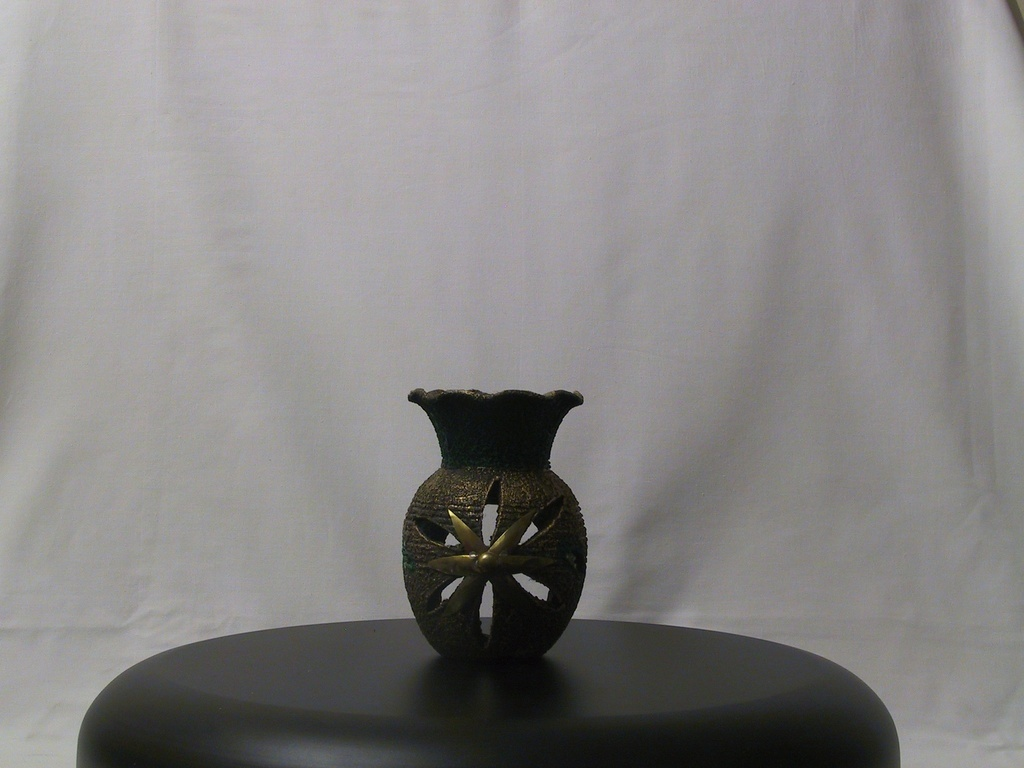
\includegraphics[width=1\columnwidth]{images/3d/2}
    \end{subfigure}%
    ~ %
    \begin{subfigure}[t]{0.19\columnwidth}
        \centering
        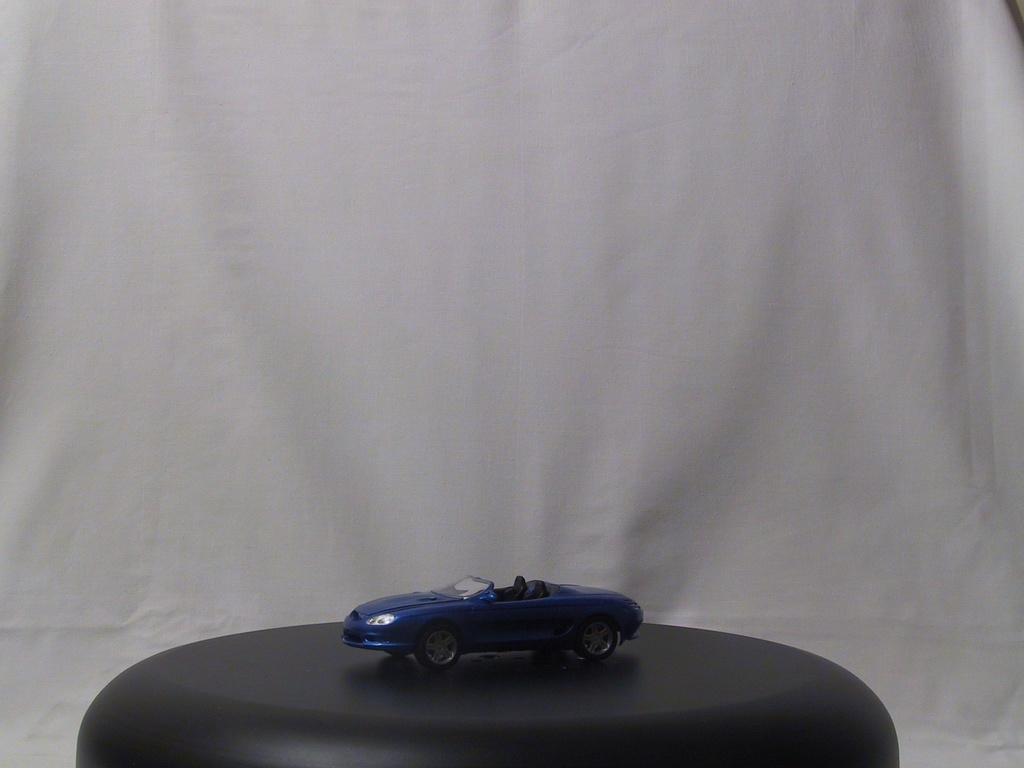
\includegraphics[width=1\columnwidth]{images/3d/3}
    \end{subfigure}%
    ~ %
    \begin{subfigure}[t]{0.19\columnwidth}
        \centering
        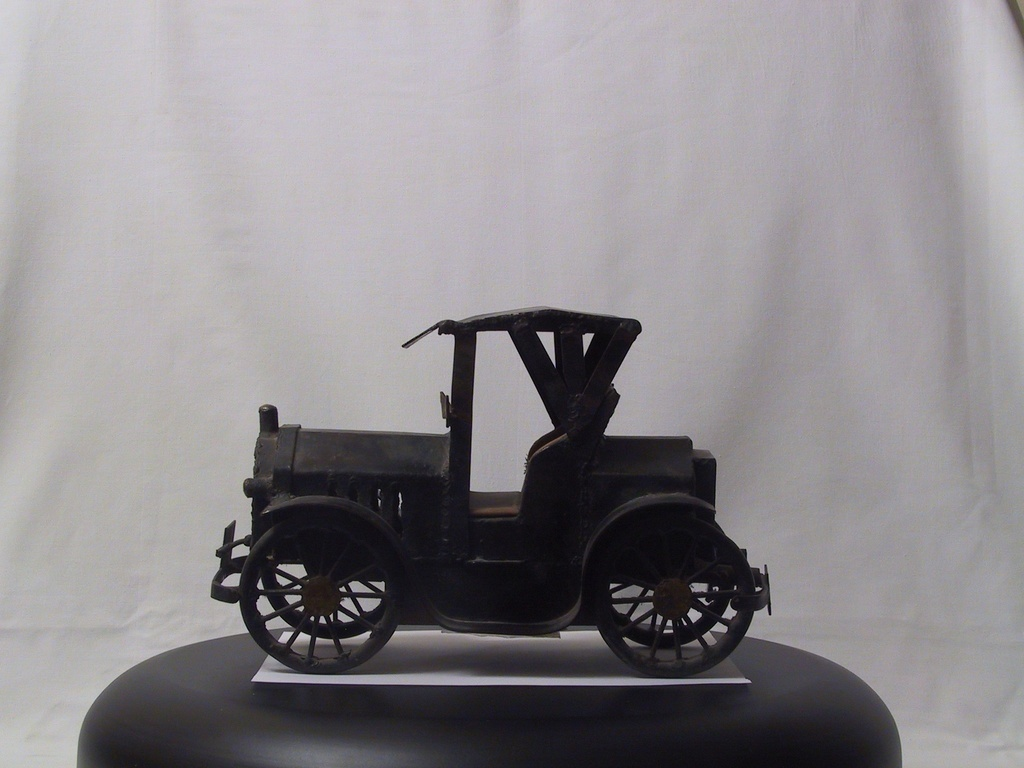
\includegraphics[width=1\columnwidth]{images/3d/4}
    \end{subfigure}%
    ~ %
    \begin{subfigure}[t]{0.19\columnwidth}
        \centering
        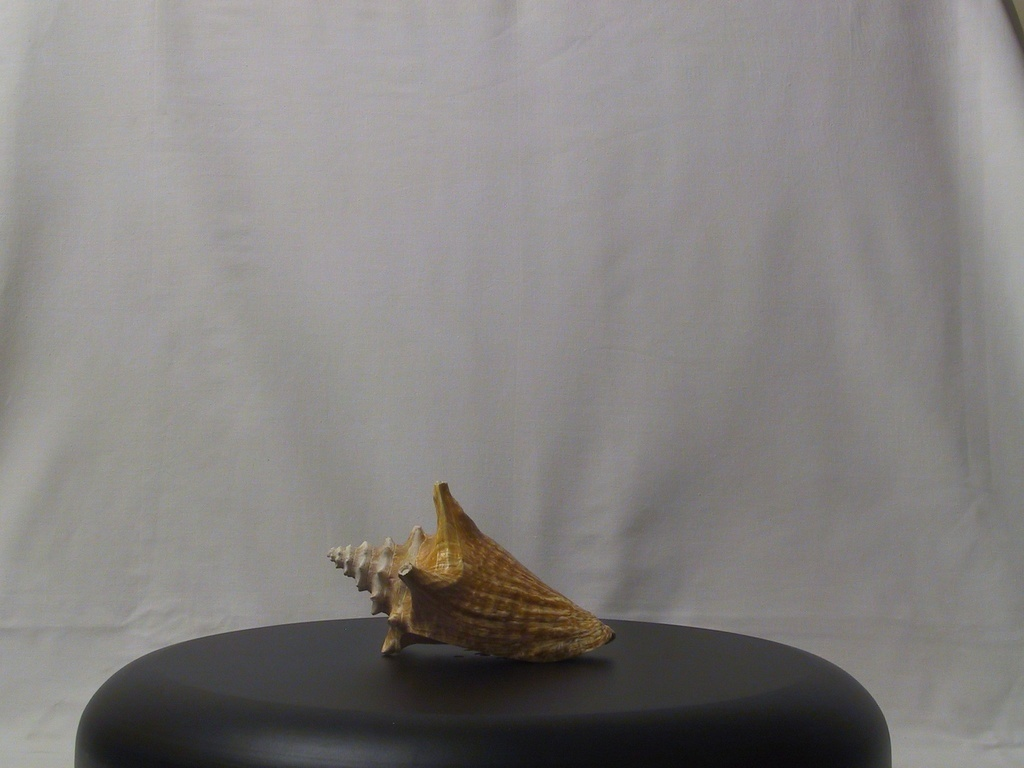
\includegraphics[width=1\columnwidth]{images/3d/5}
    \end{subfigure}%
    \vspace{1.5 mm}

    \begin{subfigure}[t]{0.19\columnwidth}
        \centering
        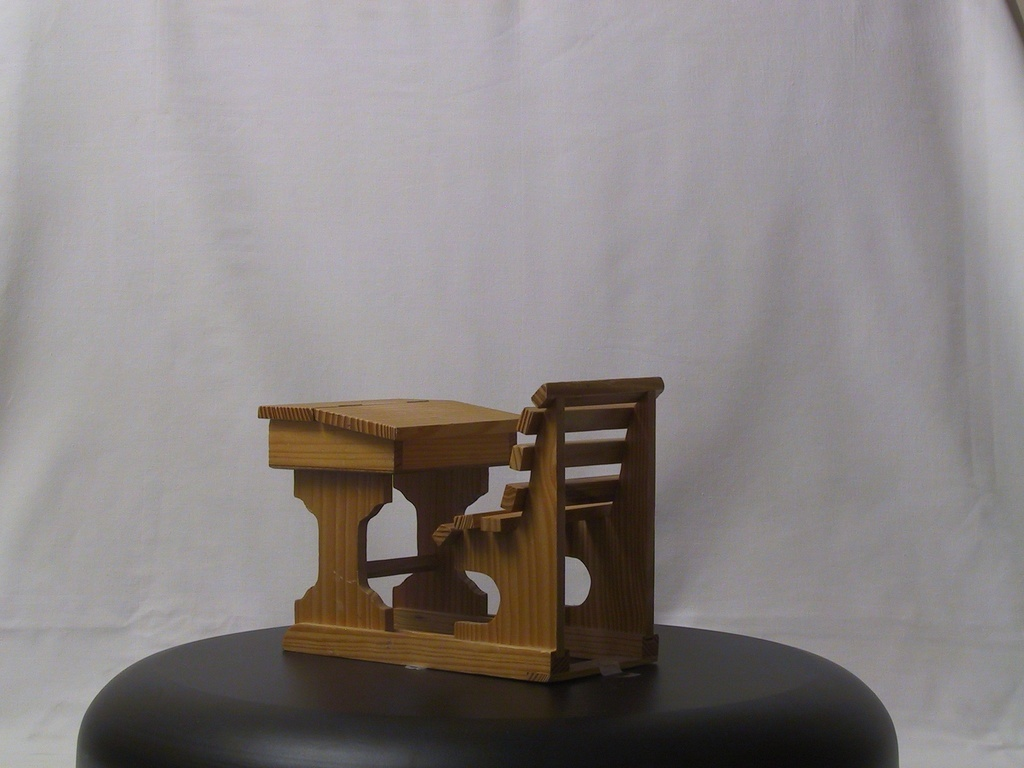
\includegraphics[width=1\columnwidth]{images/3d/6}
    \end{subfigure}%
    ~ %
    \begin{subfigure}[t]{0.19\columnwidth}
        \centering
        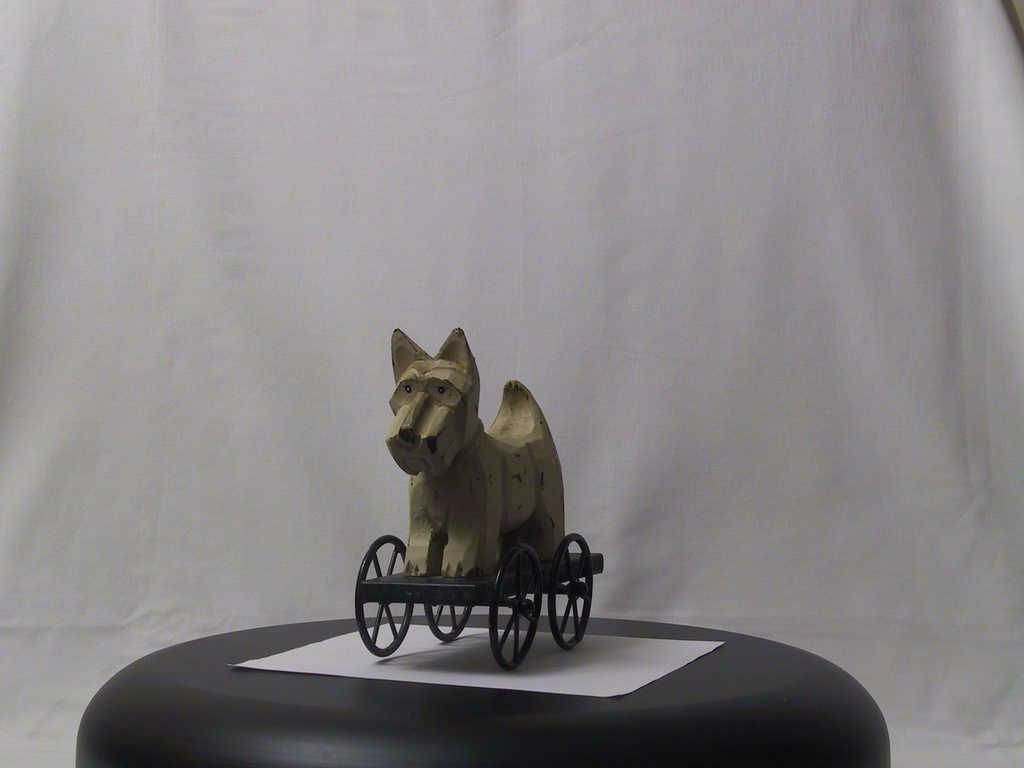
\includegraphics[width=1\columnwidth]{images/3d/7}
    \end{subfigure}%
    ~ %
    \begin{subfigure}[t]{0.19\columnwidth}
        \centering
        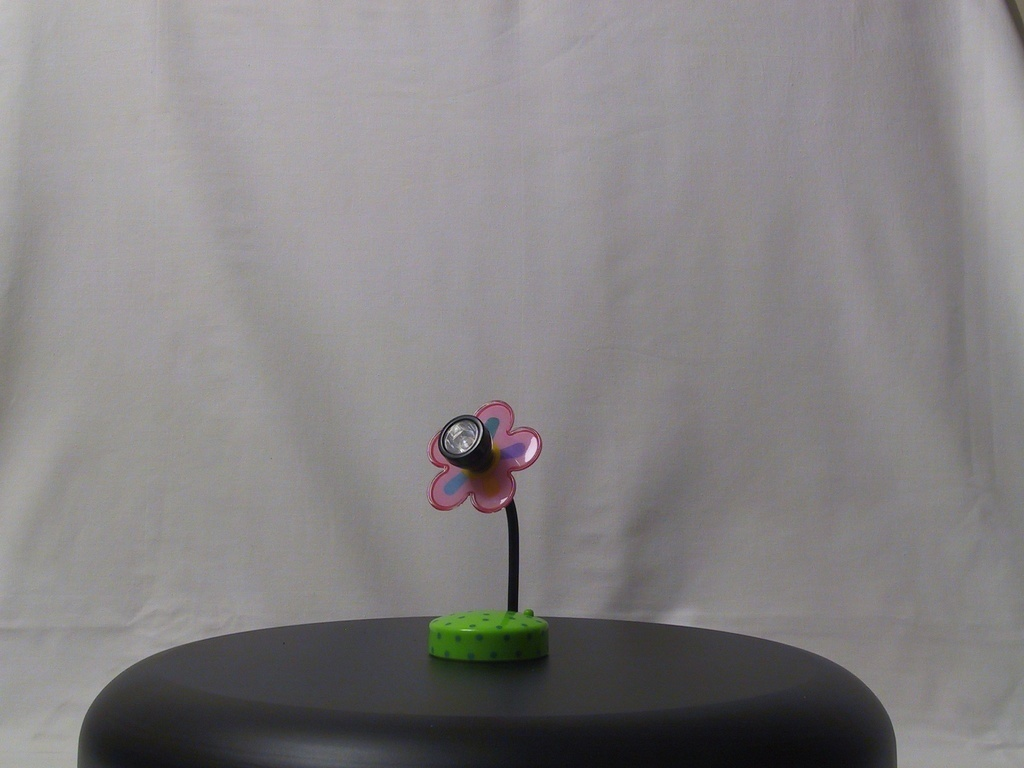
\includegraphics[width=1\columnwidth]{images/3d/8}
    \end{subfigure}%
    ~ %
    \begin{subfigure}[t]{0.19\columnwidth}
        \centering
        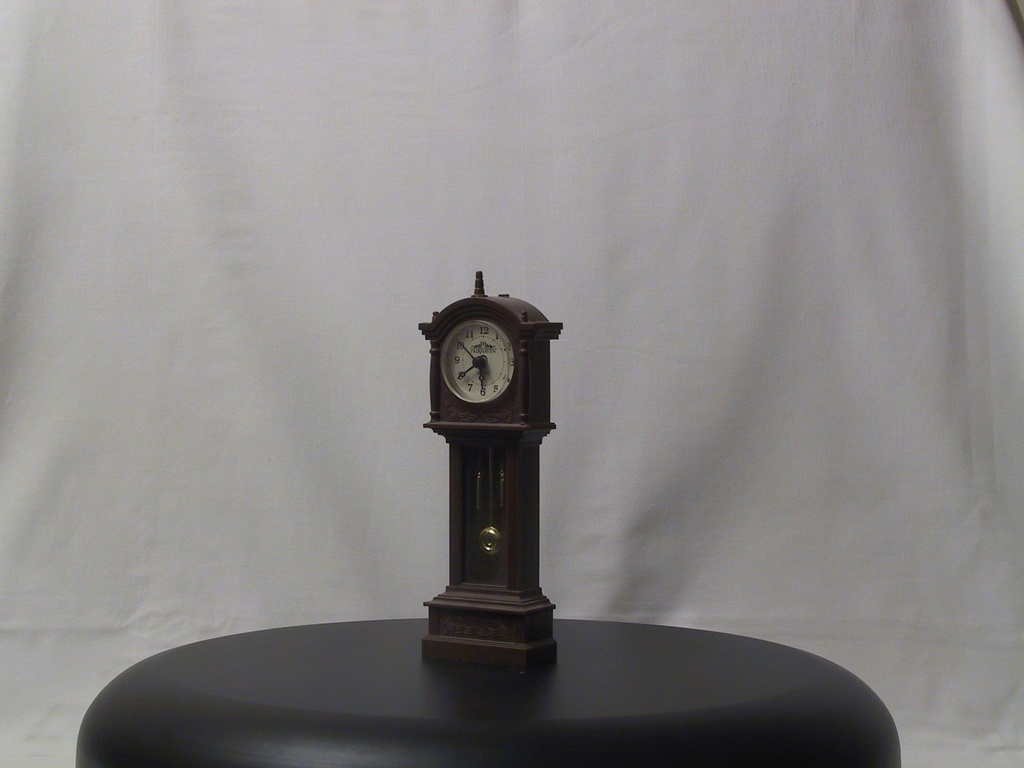
\includegraphics[width=1\columnwidth]{images/3d/9}
    \end{subfigure}%
    ~ %
    \begin{subfigure}[t]{0.19\columnwidth}
        \centering
        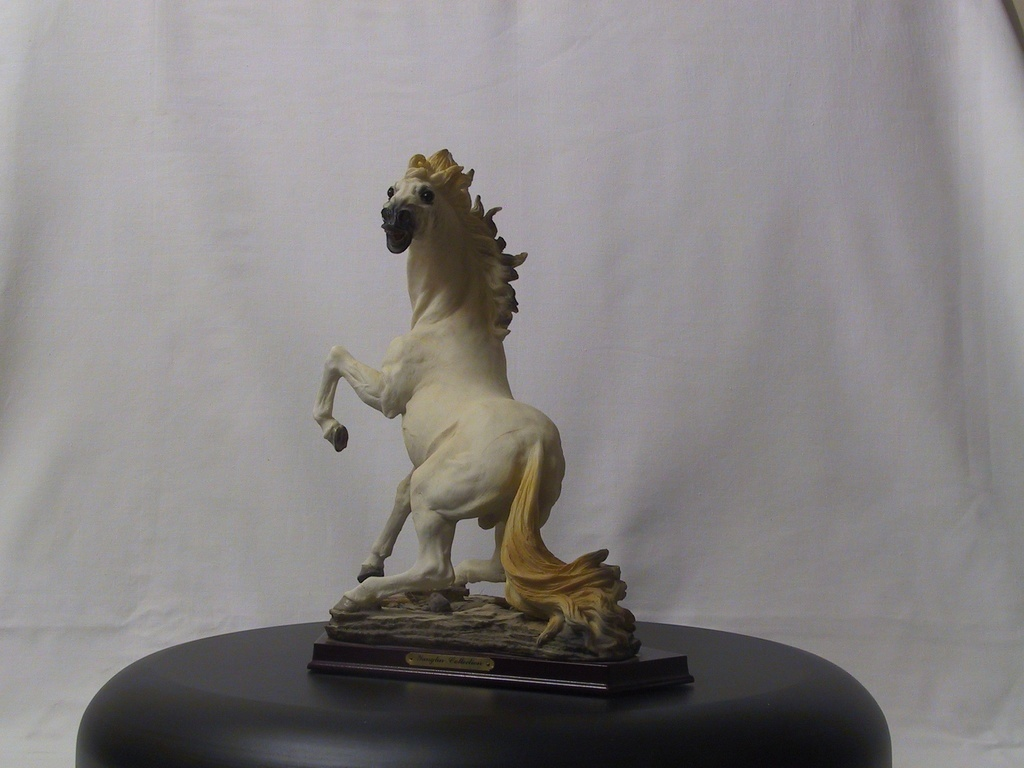
\includegraphics[width=1\columnwidth]{images/3d/10}
    \end{subfigure}%
    \vspace{1.5 mm}

    \begin{subfigure}[t]{0.19\columnwidth}
        \centering
        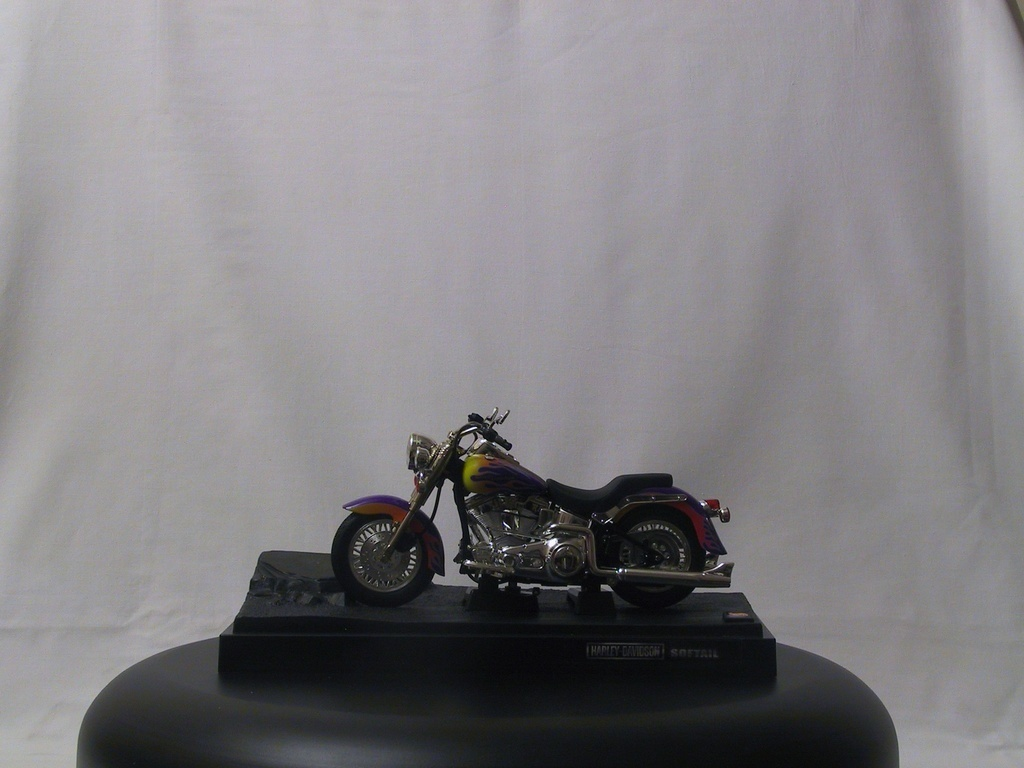
\includegraphics[width=1\columnwidth]{images/3d/11}
    \end{subfigure}%
    ~ %
    \begin{subfigure}[t]{0.19\columnwidth}
        \centering
        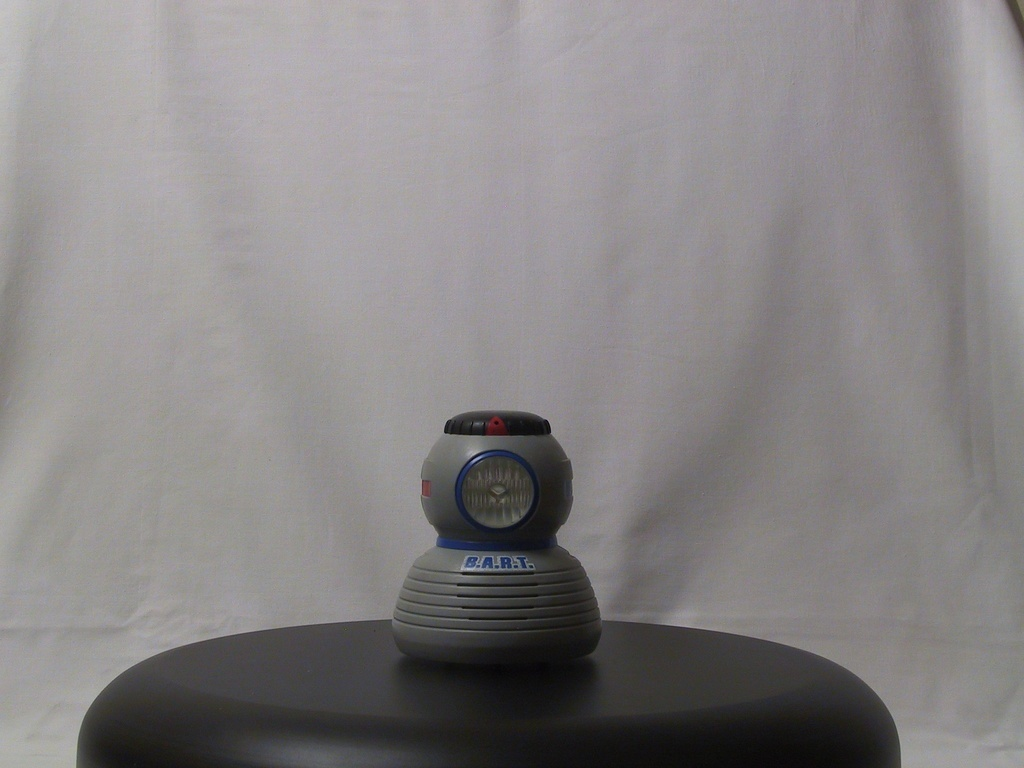
\includegraphics[width=1\columnwidth]{images/3d/12}
    \end{subfigure}%
    ~ %
    \begin{subfigure}[t]{0.19\columnwidth}
        \centering
        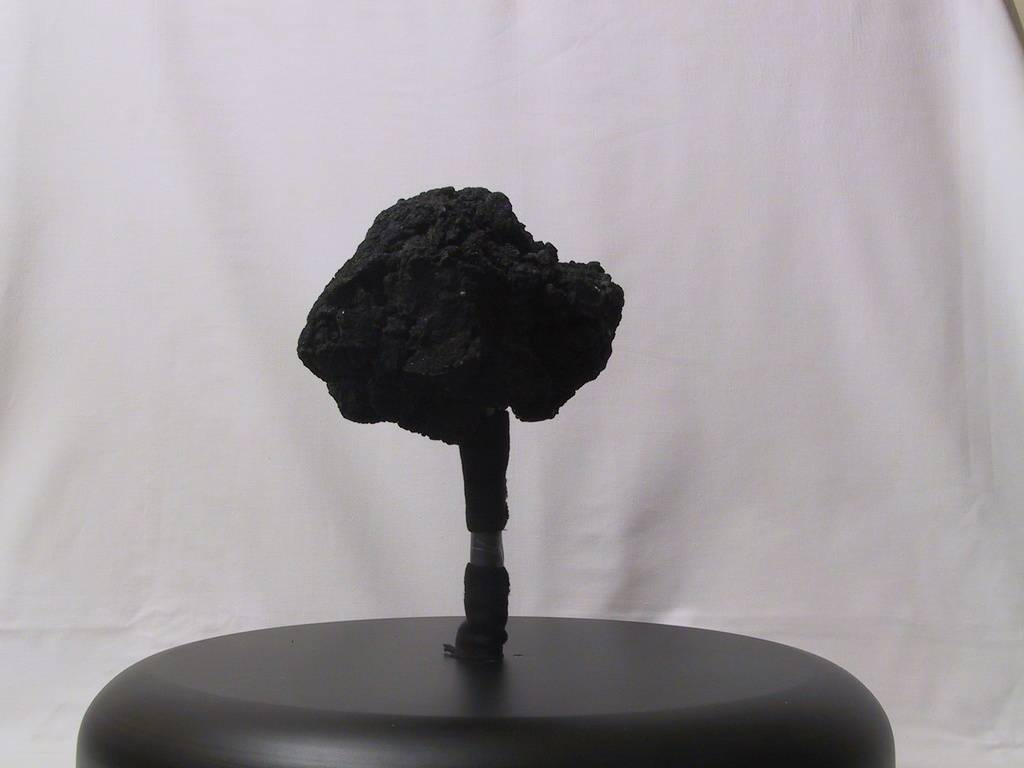
\includegraphics[width=1\columnwidth]{images/3d/13}
    \end{subfigure}%
    ~ %
    \begin{subfigure}[t]{0.19\columnwidth}
        \centering
        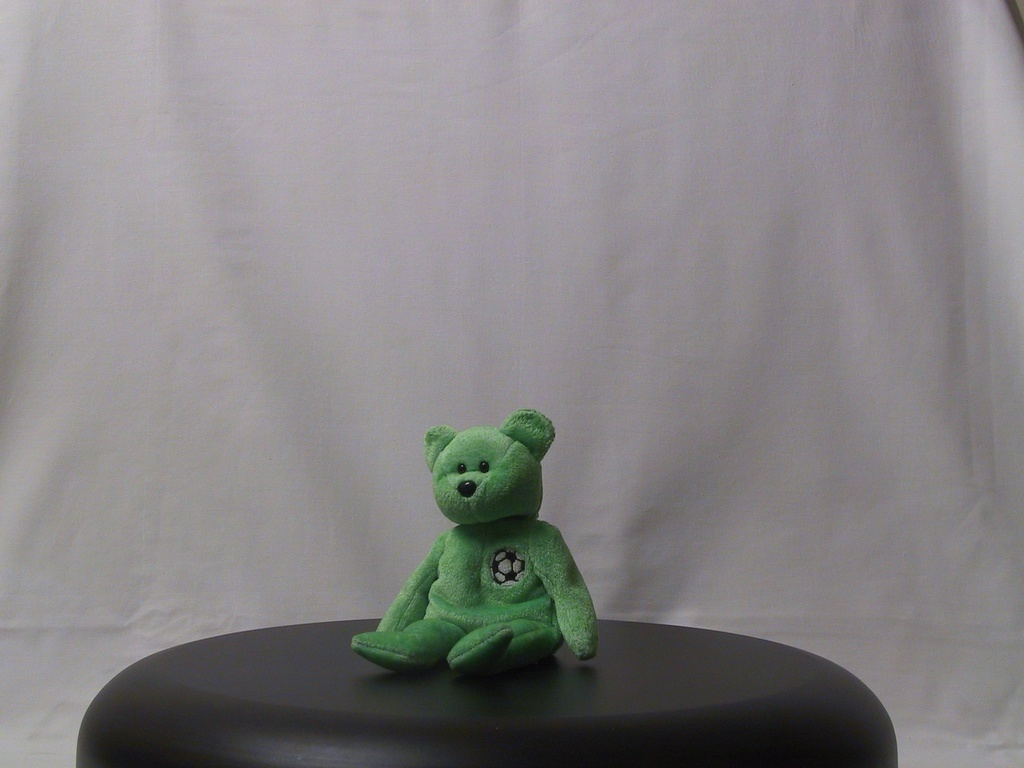
\includegraphics[width=1\columnwidth]{images/3d/14}
    \end{subfigure}%
    ~ %
    \begin{subfigure}[t]{0.19\columnwidth}
        \centering
        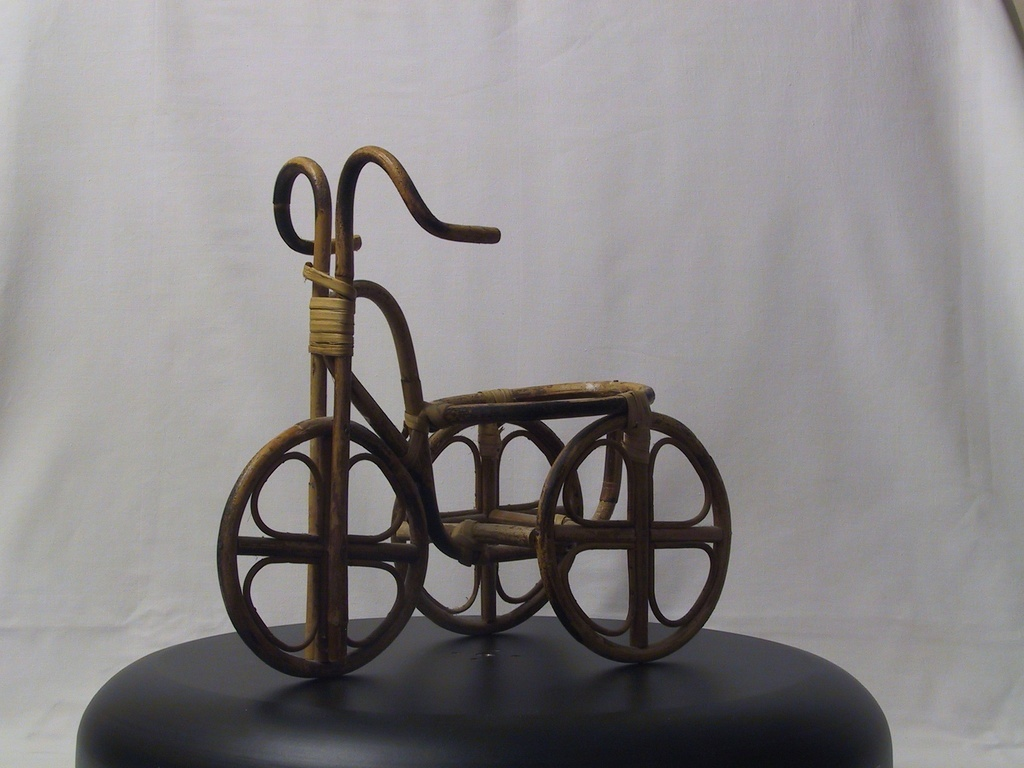
\includegraphics[width=1\columnwidth]{images/3d/15}
    \end{subfigure}%
    \vspace{1.5 mm}

    \caption{The first 15 objects from the 3D objects dataset by Moreels
    and Pietro \cite{moreels2007evaluation}}
    \label{fig:3d_objects}
\end{figure}

\begin{figure*}[ht]
	\centering
    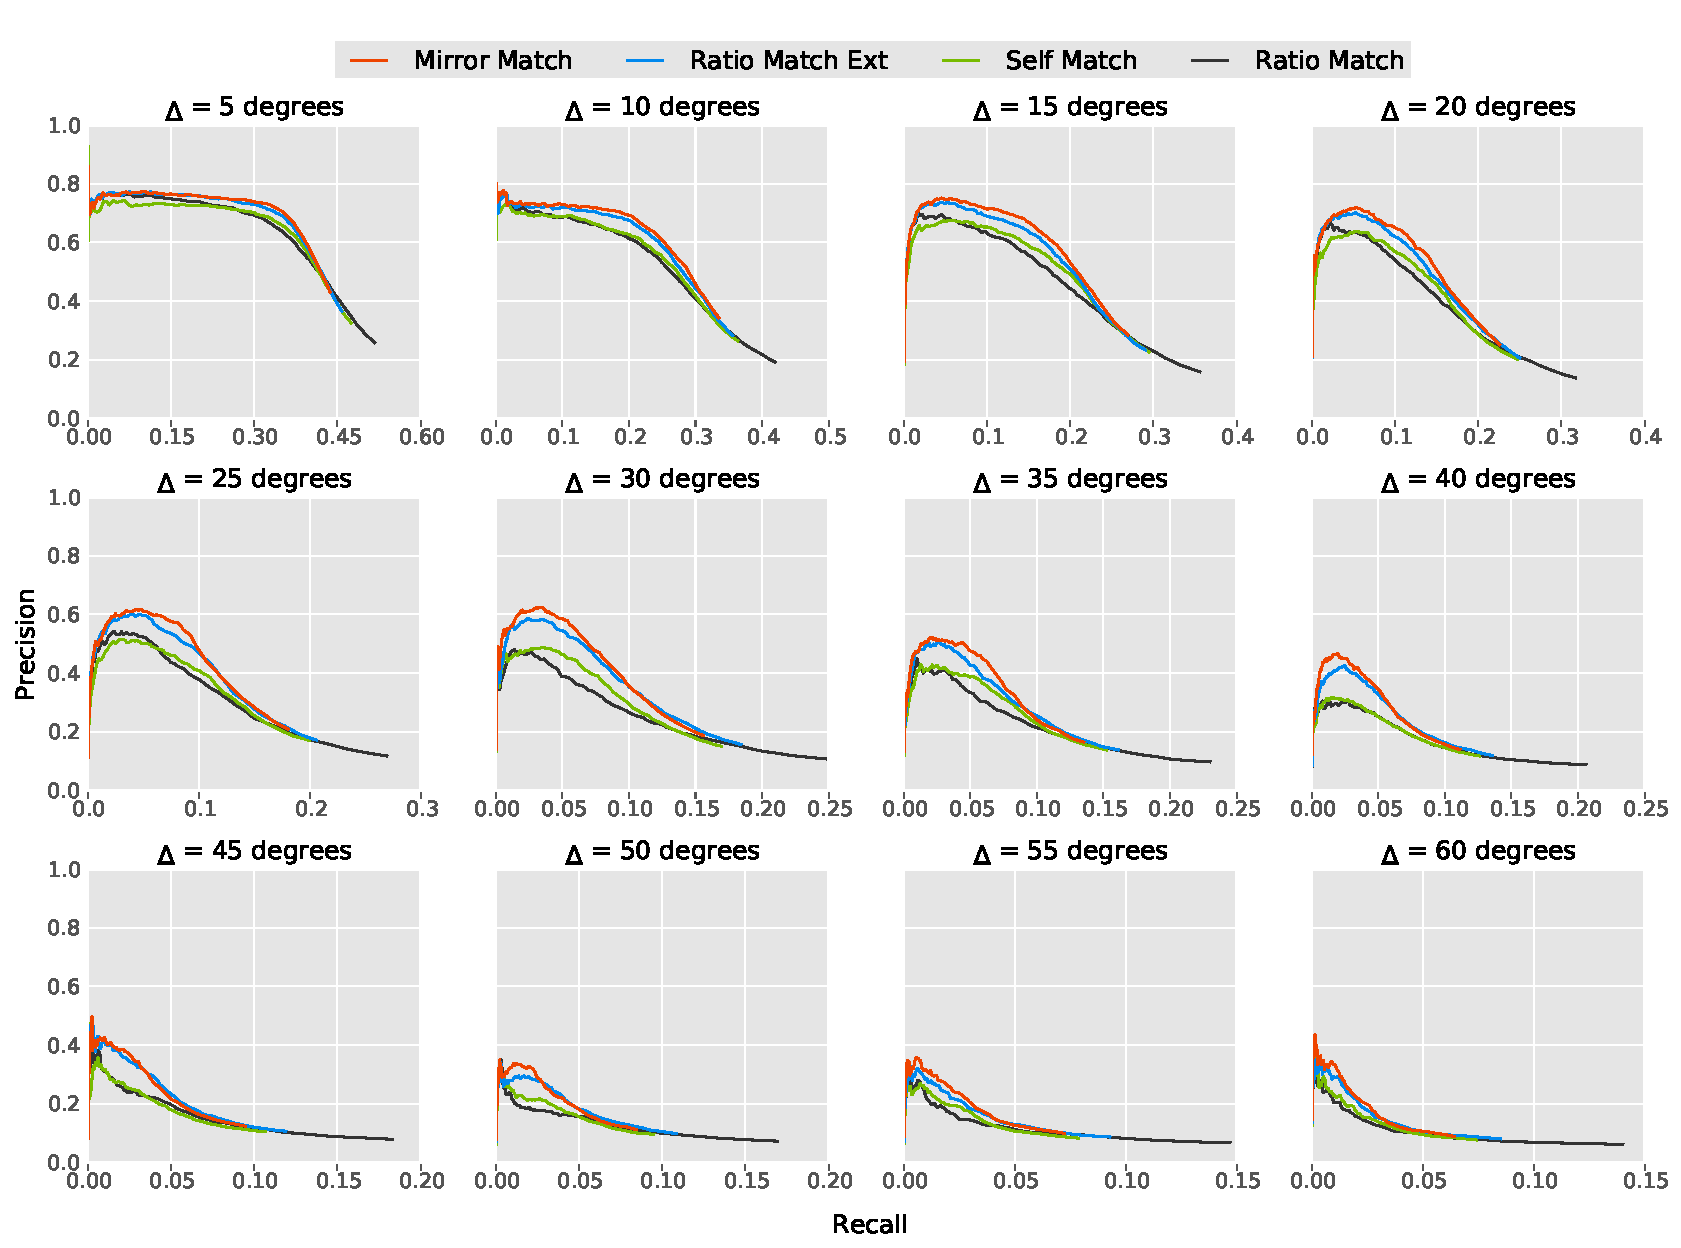
\includegraphics[width=2\columnwidth]{images/results_all_objects}
    \caption{Accumulated results from the 3D objects dataset. Each plot 
    contains data accumulated from 84 objects photographed under 3 
different lighting conditions.}
    \label{fig:all_objects}
\end{figure*}


The 3D objects dataset allows us to experimentally comparing matching 
algorithms over a large range of object and surface types rotated on a 
turnstile and photographed from every 5 degree turn. We used images of 
84 different objects under three different lighting conditions at 12 
different angle intervals conducting experiments with a total of 3024 
image pairs.  To validate matches, Moreels and Pietro propose a method 
to that will validate a match as a true or false correspondence using 
epipolar constraints \cite[p.  266]{moreels2007evaluation}.  Their 
method is outlined in Figure~\ref{fig:frog}.  According to their 
experiments these constraints are sufficient to reduce the error rate 
recognizing true correspondences to $2\%$. We have used their proposed 
method to evaluate the precision and recall of the framework methods.

To compute the total number of possible correspondences we took each 
feature in a \emph{query image} and counted how many of them had a 
feature in the \emph{target image} which would satisfy the epipolar 
constraints outlined above. In the experiments on 3D objects features 
with no correspondences were not included in the set of features used to 
test the matching algorithms to avoid matching non-moving background and 
foreground objects.

We evaluated the 4 matching algorithms on the 3D objects dataset by 
matching images at different angular intervals. For each object we 
picked the \emph{query} image as the image taken at 10 degrees rotation 
for calibration stability.  We then proceeded to match this image with 
the same object turned an additional $d$ degrees, $d \in \{5, 10, 
\ldots, 60\}$.  For every angle interval we compaired images taken under 
3 different lighting conditions as provided by the dataset.
We included all objects in the database for which photos at 5 degree 
angle intervals were available except for the ``Rooster'' and ``Sponge'' 
objects due to image irregularities. For each plot we show the 
accumulated results on all 3D objects, weighed by the number of possible 
true correspondences for the particular object. This ensures that each 
object contributes equally to the final result despite some objects
resulting in disproportionally more matches than others.

The results can be seen in Figure~\ref{fig:all_objects}. In the figure
we see the performance of the different matching methods in our proposed
framework for $12$ increasingly bigger rotations. The results are shown
in a precision / recall plot to make it easy to compare performance in
terms of precision at similar levels of recall. For the application of
feature matching it is important to keep in mind that for many
applications, such as image stitching, object and scene recognition and
near duplicate detection, precision is much more important than recall,
since a handfull of highly reliable correspondences tells us much more
about the similarity of image components than a high number of imprecise
matches. For applications where we intent to combine one of the
algorithms with a geometric method, we would ideally like for it to
produce results with a high recall that can then be further filtered by
a geometric method.

For objects in the top row rotated between $5$ and $20$ degrees we see a 
gradual increase in the performance gap between the methods as the angle 
increases.  \emph{Ratio-Match} and \emph{Self-Match} show similar 
results while \emph{Mirror-Match} and \emph{Ratio-Match-Ext} outperform 
the them, showing the advantage of composing the \emph{proposed set} of 
features from both images. \emph{Mirror-Match} show performance which is 
consistently slightly better than \emph{Ratio-Match-Ext}. In general we 
see the largest performance improvements at lower recall and a 
convergence of precision at higher recall. This is expected since a 
higher recall is a direct consequence of a more lenient threshold and as
we let the threshold approach $1$ we lose the benefits of thresholding 
on the \emph{uniqueness ratio} the methods all start approximating the 
results of a simple nearest neighbor match. However for all but 
\emph{Ratio-Match} the features with better matches within the same 
image are still weeded out, which explains the tail end of 
\emph{Ratio-Match} at high recall where the other algorithms no longer 
have results. As we demonstrated in \cite{arnfred2013mirror} the removal 
of within-image matches improves performance on image pairs with partial 
or no overlap. For no overlap we would expect a matching algorithm to 
reject matches within regions that have no matching counterparts in the 
other image.

In the middle row featuring rotations of between $25$ and $40$ degrees 
we see the strongest improvement of \emph{Mirror-Match} compared to 
\emph{Ratio-Match} generally peaking at around
a $20$ percentage-point increase in precision. Finally the the performance
gain decreases as we further increase the rotation to between $45$ and 
$60$. We suspect that this is partly because assumption \#2 that a 
descriptor is well behaved and match best with a descriptor of a true 
correspondence stops being valid when the images are transformed beyond 
a certain level of recognizability.

To summarize, the methods perform as predicted on the 3D Objects dataset
with \emph{Mirror-Match} in general performing better than 
\emph{Ratio-Match-Ext} which in turn was performing better than 
\emph{Ratio-Match}. The experimental results also show that 
\emph{Self-Match} overall perform equal to or better than 
\emph{Ratio-Match}.

\subsection{Descriptor evaluation}
\label{label:desc}

\begin{figure*}[t]
    \centering
    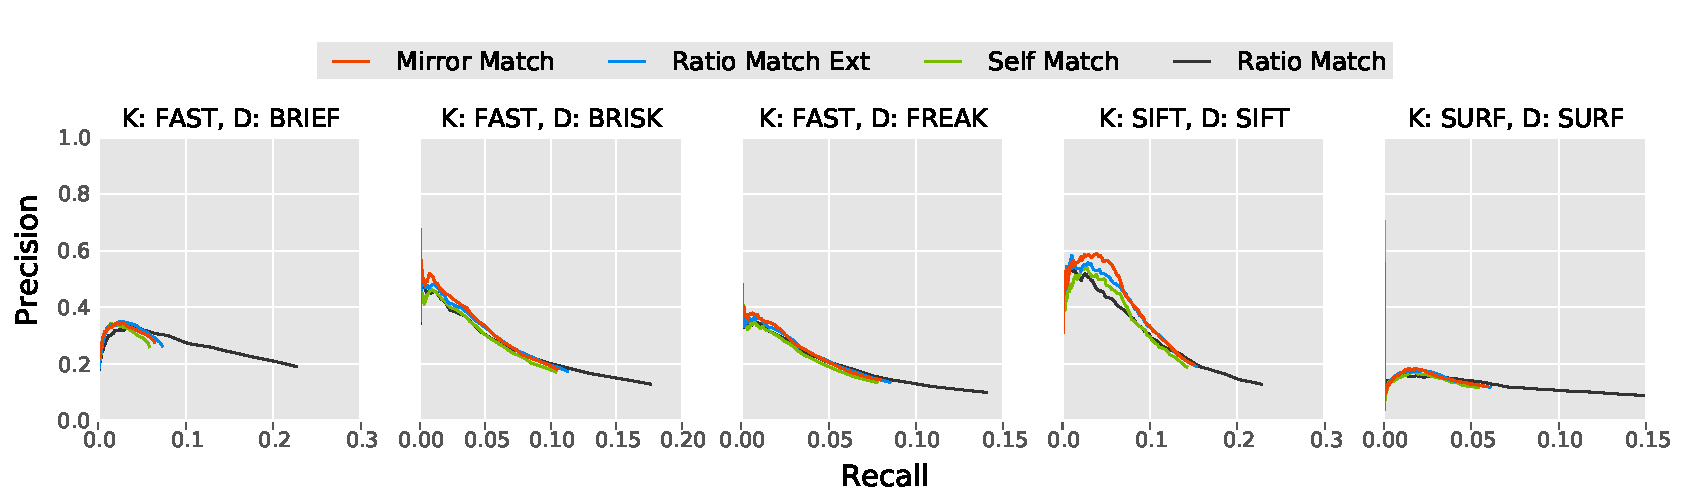
\includegraphics[width=2\columnwidth]{images/results_descriptors_imageset1}
    \caption{Keypoint / Descriptor combinations measured on 15 pairs of 
    photos of 3D objects taken 15 degrees apart. K = Keypoint, D = 
Descriptor.}
    \label{fig:descriptors}
\end{figure*}

To evaluate whether the improvement gains shown with the SIFT descriptor 
translates to other feature descriptors such as SURF \cite{bay2006surf} 
or binary features such as BRIEF \cite{calonder2010brief}, BRISK 
\cite{leutenegger2011brisk} or FREAK \cite{alahi2012freak} we evaluated 
the different descriptors on the 3D objects data set.  For the binary 
features they were each paired with the FAST feature detector while SIFT 
and SURF were tested with their respective feature detectors.  For each 
keypoint detector and feature descriptor pair we used the standard 
implementation from OpenCV 2.4.6.

The descriptors were evaluated on 15 images of the 3D object dataset 
with a fixed angle offset of 25 degrees (pictured in 
Figure~\ref{fig:3d_objects}).  The evaluation was otherwise performed as
in the general evaluation of 3D Objects, and the data presented is 
accumulated over the 15 objects, each set of results weighted by the 
possible amount of correspondences.

The results can be seen in Figure~\ref{fig:descriptors} and shows a 
clear difference in the variance of matching method performance in 
between SIFT and the rest of the descriptors. The performance of 
\emph{Mirror-Match} using SIFT shows a clear increase in precision over 
\emph{Ratio-Match} at equal recall levels. For other descriptors the 
improvement is much less pronounced.  For the case of SURF, BRISK and 
BRIEF we see a small improvement in precision using \emph{Mirror-Match} 
over \emph{Ratio-Match} and \emph{Ratio-Match-ext} while FREAK yields 
similar results no matter what algorithm is used. For all descriptors it 
is the case that \emph{Self-Match} performs equally well to 
\emph{Ratio-Match}.

Part of the explanation behind this difference between SIFT and the 
other descriptors can be found by looking at the recall rate in the case
of for example SURF\@. Given the same amount of possible matches, 
\emph{Ratio-Match} in the case of SURF spans a larger range of recall.  
Since all other methods filter out matches that are better matched 
within the same image but show no increase in precision, we can conclude 
that correct matches are discarded because there are better matches 
within the same image. This violates assumption \#2 stating that a 
descriptor is well behaved and match best with a descriptor of a true 
correspondence. This means that for this particular evaluation case SURF 
and the binary features tested are not sufficiently discriminative to 
provide a viable case for preferring \emph{Mirror-Match} over 
\emph{Ratio-Match}.

\subsection{Performance}

In terms of computational complexity the algorithms can be implemented 
in $O(n\log n)$, if we assume that both the \emph{query} and the 
\emph{target} image has $n$ feature points. For a target image with $m$ 
features where $m$ is significantly different from $n$ the complexities 
are as noted in Table~\ref{table:running_times}. In practice the constant factors 
involved in the actual matching of two images with approximately the 
same amount of feature points are usually small enough that all the 
algorithms run at a similar speed. To illustrate 
Table~\ref{table:running_times} contains the running times as measured 
while matching 15 3D objects under three different lighting conditions 
($42$ image pairs were matched in total). The running times are averaged 
over three separate runs of each algorithm implemented using the same 
data structures and libraries in Python. 

\begin{table}[htb]
\caption{Complexity and running times tested on 45 image pairs with average $n = 237$ and average $m = 247$ 
as tested on a Intel\textregistered\ Core\texttrademark\ i5-3550 CPU @ 
3.30~GHz with 8~GB memory.}
\label{table:running_times}
	\centering
%	\small
    \begin{tabular}{{l}{l}{l}}
    Algorithm & Complexity & Running Time\\
    \hline
    \noalign{\smallskip}
    %
    \emph{Self-Match} & $O(n\log(nm))$ & 118s  \\
    %\emph{Self-Match-Ext} & $O(n\log(n(n+m)))$ & 109s\\
    \emph{Ratio-Match} & $O(n\log(m))$ & 114s\\
    \emph{Ratio-Match-Ext} & $O(n\log(n+m))$ & 112s\\
    %\emph{Both-Match} & $O(n\log(n(n+m)))$ & 116s\\
    \emph{Mirror-Match} & $O(n\log(n+m))$ & 110s \\
    \hline
\end{tabular}
\end{table}

\subsection{Extending to multiple target images}
%
When we match a query image against multiple target images as seen in 
for example image stitching, assumption \#1 that any feature in the 
query image has at most 1 real correspondence in the set of target 
features is no longer true. It might be the case that two target images 
contain the same real object which yields two target features that are 
both real correspondences. In this case calculating the \emph{uniqueness 
ratio} by dividing the distance of one real correspondence with the 
distance to another renders it entirely useless if the two features are 
found in sets where there might be more than one correct 
correspondences.

Brown et al.\ \cite{brown2005multi} proposes calculating the uniqueness 
ratio by taking the average of the $n$ nearest neighbors in each of the 
$n$ target images. Since their particular case deals with images that 
are aligned horizontally one after the other, this approach is not 
flawed per se. However for the more general case of $n$ target images 
with an unknown amount of overlaps in the target group, their approach 
would not work since several features in the target group could possible 
be a correct correspondence. 

This leaves us with two alternatives. Either we match the query image to 
every target image individually or we use a matching strategy where the 
\emph{baseline set} is guaranteed not to contain any real 
correspondences. \emph{Self-Match} provides such a set, since the 
\emph{baseline set} of \emph{Self-Match} only contains features in the 
query image itself. In addition, matching a query image to $n$ target 
images with \emph{Self-Match} is vastly faster than matching the query 
image to every target image: If we for the sake of simplicity assume 
that every of the $n$ images has $k$ features then matching the query 
image to all $n$ images can be done in $O(nklog(k))$ using a metric 
tree. However, matching with \emph{Self-Match} is done in $O(klog(nk)) =
O(klog(n) + klog(k))$.

\section{Conclusion}
\label{S:Summary}

We have proposed a framework of matching methods building on the ideas 
behind \emph{Ratio-Match} and \emph{Mirror-Match} introducing the 
variations \emph{Self-Match} and \emph{Ratio-Match-Ext}. We proved that 
in terms of precision and recall \emph{Mirror-Match} performs better or 
equal to \emph{Ratio-Match-Ext} which in turn performs better or equal 
to \emph{Ratio-Match} under three common assumptions.

From an evaluation using images of rotated 3D objects we have shown that
the theoretical conclusions are reflected in experimental data with 
\emph{Mirror-Match} often outperforming \emph{Ratio-Match}
significantly over 3024 image pairs. This performance gain comes free in 
terms of both computational complexity as well as actual time 
consumption as measured over 45 image pairs. Finally evaluations across 
several different descriptors show that the gains in performance are 
tied to descriptor performance with significantly smaller gains occuring 
with descriptors that are less performant.

With the framework we introduced three simple methods that are all 
applicable in situations where \emph{Ratio-Match} is currently used.  
\emph{Self-Match} is on par with \emph{Ratio-Match} across all 
evaluations but can be applied when matching multiple overlapping 
images. \emph{Ratio-Match-Ext} and \emph{Mirror-Match} on the other hand 
can easily replace \emph{Ratio-Match} without any performance penalty 
and with an increase in precision but are both limited to matching 
image pairs like \emph{Ratio-Match}.

\appendix

\subsection{Proof of equivalence of Self-Match and Self-Match-Ext}
\label{A:self}

In this appendix we prove the equivalence between \emph{Self-Match} and 
\emph{Self-Match-Ext}. To do this, we look at the nearest neighbor 
$f_{nn}$ of every query feature $f_{q}$ and consider the two cases of 
$f_{nn} \in F_{query}$ and $f_{nn} \in
F_{target}$. For $f_{nn} \in F_{target}$ the uniqueness ratio of 
\emph{Self-Match-Ext} is:
\begin{align*}
    r &= \text{r}(f_{q}, F_{proposed}, F_{baseline}) \\
        &= \text{r}(f_{q}, F_{query} \cup F_{target}, F_{baseline})\\
        &= \text{r}(f_{q}, F_{target}, F_{baseline})
\end{align*}

Since $F_{proposed} = F_{target}$ for \emph{Self-Match} this shows that
when the nearest neighbor is found in the target image, the two 
algorithms behave identically. For $f_{nn} \in F_{query}$ we know that 
the best match for the query feature is in the query image itself. Since 
neither algorithm returns a correspondence within the same image, they 
also behave identically for this case. This proves that for any set of 
\emph{query features} \emph{Self-Match} returns the same matches as 
\emph{Self-Match-Ext}.

\subsection{Proof of equivalence of Both-Match and Mirror-Match}
\label{A:mirror}

In this appendix we prove the equivalence between \emph{Both-Match} and 
\emph{Mirror-Match}. This proof is almost identical to the equivalence 
proof between \emph{Self-Match} and \emph{Self-Match-Ext}. To prove 
this, we look at the nearest neighbor $f_{nn}$ of every query feature 
$f_{q}$ and consider the two cases of $f_{nn} \in F_{query}$ and $f_{nn} 
\in
F_{target}$. For $f_{nn} \in F_{target}$ the uniqueness ratio of 
\emph{Mirror-Match} is:
\begin{align*}
    r &= \text{r}(f_{q}, F_{proposed}, F_{baseline}) \\
        &= \text{r}(f_{q}, F_{query} \cup F_{target}, F_{baseline})\\
        &= \text{r}(f_{q}, F_{target}, F_{baseline})
\end{align*}

Since $F_{proposed} = F_{target}$ for \emph{Both-Match} this shows that
when the nearest neighbor is found in the target image, the two 
algorithms behave identically. For $f_{nn} \in F_{query}$ we know that 
the best match for the query feature is in the query image itself. Since 
neither algorithm returns a correspondence within the same image, they 
also behave identically for this case. This proves that for any set of 
\emph{query features} \emph{Both-Match} returns the same matches as 
\emph{Mirror-Match}.


\bibliographystyle{IEEEtran}
\bibliography{tail/bibliography}
\end{document}


